\documentclass[a4paper,11pt]{article}
%\usepackage{tocvsec2}
%\usepackage{titletoc}
\usepackage{titlesec}
\usepackage{enumitem}%let description environment new line description content
\usepackage{ifthen}
\usepackage{verbatim}
\usepackage{multicol}
\usepackage{longtable}
\usepackage{lmodern}
\usepackage[T1]{fontenc}
\usepackage{textcomp}
\usepackage{underscore}%正文使用_
\usepackage{fancyhdr}
\pagestyle{fancy}
\usepackage[titletoc]{appendix}
\usepackage{makeidx}%索引
\usepackage[iso]{isodateo}%控制\today的格式
\usepackage{tikz}
\usetikzlibrary{patterns}
\usepackage{graphics}
\usepackage{listings}
\usepackage{xcolor}
\lstset{language=C,
    breaklines=true,
    extendedchars=false,
    breakautoindent=true,
    breakindent=10pt,
    numbers=left, 
    basicstyle=\tiny,%\scriptsize,
    numberstyle=\tiny,
    keywordstyle=\tiny\color{blue!70}, 
    commentstyle=\color{red!50!green!50!blue!50},
    escapeinside={(*@}{@*)}
    %  frame=shadowbox,
  %  rulesepcolor=\color{red!20!green!20!blue!20}
  }
\lstdefinelanguage{KC}{language={C},morekeywords={uint32_t, size_t}}
\usepackage[CJKbookmarks=true, bookmarksnumbered=true,
colorlinks=true,% frenchlinks=true, raiselinks=true, xetex,, linktocpage=true 
citecolor=magenta, linkcolor=blue]{hyperref}
%\usepackage[CJKbookmarks=true, bookmarksnumbered=true,
%colorlinks=false, citecolor=magenta]{hyperref}
\usepackage{xeCJK}
\setCJKmainfont{AR PL UKai CN}
\setCJKmonofont{文泉驿等宽正黑}
%\setCJKfamilyfont{AR PL UKai CN}{kai}
\setmainfont{DejaVu Sans}
\title{Android Binder From Deep}
\author{Leo shecenon@gmail.com}
\date{\today}

\makeindex 

\begin{document}
\maketitle
\renewcommand{\refname}{参考文献}
\renewcommand\contentsname{目录}
\renewcommand\listfigurename{插图目录}
\renewcommand\listtablename{表格目录}
\renewcommand\indexname{索引}
\renewcommand\appendixname{附录}
\renewcommand\figurename{图}
\renewcommand\tablename{表}
\renewcommand{\lstlistlistingname}{代码列表集}
\renewcommand{\lstlistingname}{代码}

%\renewcommand\thefootnote{\thempfootnote}

\setdescription{labelsep=\textwidth}
%\setlength{\multicolsep}{3pt} 
%\multicolsep=\skip59
\setlength{\columnsep}{.8cm}
%\titlecontents{section}[1.5em]{}{\thecontentslabel}{}{\dotfill \contentspage}
%\titlecontents{section}[1.5em]{\color{blue}\normalsize\addvspace{1.0ex}}{\contentslabel{2em}\hspace∗{−0.0em}}{\hspace∗{−3.3em}}{\color{black}\titlerule ∗[0.8pc]{}\contentspage}
\setlength{\parskip}{1ex}
\headheight13.6pt
\tableofcontents
\newcommand{\various}[1]{{\color{cyan}\textit{#1}}}
\newcommand{\binder}{{\color{red}binder }}
\makeatletter
\newcommand{\figcaption}{\def\@captype{figure}\caption}
\newcommand{\tabcaption}{\def\@captype{table}\caption}
\makeatother

\setlength{\leftmargin}{1.2em}     %左边界
\setlength{\parsep}{0ex}         %段落间距
\setlength{\topsep}{1ex}         %列表到上下文的垂直距离
\setlength{\itemsep}{0.5ex}        %条目间距
\setlength{\labelsep}{0.3em}     %标号和列表项之间的距离,默认0.5em
\setlength{\itemindent}{1.1em}    %标签缩进量
\setlength{\listparindent}{0em} %段落缩进量

%\hypersetup{CJKbookmarks=true}
\section{Binder基本架构}
简单的说,binder就是个跨进程的指针。现代操作系统里,一个进程的地址空间是确定的
,地址是没有二义性的,进程里的一个指针就对应一个内存地址,不可能同时对应到多个
地址,给定一个指针,就能获得想要的东西。但跨进程的情况下,事情就完全不一样了,
不同进程的线性地址空间都是一样的,一个进程里的指针放到另一个进程里,就是完全不
同的东西了。要实现跨进程的指针,就必须通过操作系统层,只有在系统底层才能将一个
进程里的地址映射到另一个进程里的地址,这也就是 Binder驱动所做的事情。跨进程的
指针(以下直接记为 \binder )有两种存在方式,一是在本地进程里的存在,一是在远程
进程里的存在,驱动所做的其实就是实现这两种存在方式的转换。当进程 A 要使用一个
活在进程 B 里的 \binder 时,驱动根据这个 \binder 在进程 A 中的表示,找到这个
\binder 的本地进程表示,获取其所在进程和实际指针,然后让它来完成进程A的需求。

由于\binder 有着这两种不同的存在方式,写程序时得区分\binder 是不是本进程的指针,
这就给用户带来了很多麻烦,失去了跨进程指针的本来意义。为了让用户接口统一,不论
是用本地的还是用远程的指针,都使用一套接口,c++/java 粉墨登场。在这两种高级语
言里,这个跨进程的指针实际上是一个对象的指针,所以\binder 事实上就升级成了跨进
程的对象,用户只需要调用对象的函数就能使用\binder ,不必关心这个对象是活在本进
程的还是活在别的进程中。实现上,提炼这个对象的基本操作成基本接口,分别用两个子
类继承之,一个用来实现本地对象,一个用来实现远程对象,用户使用时用基本接口就行
了,不必关心对象所在进程,底下的细节由 c++的Binder库来完成。另一方面,由于 JNI
的存在,android 应用程序赖以生存的 java 层Binder实际上是通过调用 c++ 实现的。
因此,android的 Binder ,一半功劳属于Binder 驱动\cite{BinderKernel},而另一半功
劳则属于 c++的 Binder 库\cite{BinderLibrary},这个库的具体细节以后有空再写。

\binder 的两种存在方式,一是本地进程里的存在方式,在本地进程里来看,很简单,用
他自己的一个指针就能表示,但是从驱动角度来看,光一个进程内指针是不够的,驱动需
要区分所有进程的指针,必须再加上一个参数,由于进程本身是操作系统独一无二的,所
以驱动里用进程和进程内指针这两个参数就能唯一代表一个 \binder。而 \binder 在远
程进程中的存在,驱动里也是用二元组来表示的,第一维依旧是进程,驱动必须知道这个
表示是为哪个远程进程维护的,第二维是一个数,叫做ref, handle, desc都行(以下记
作 desc,免得混淆),它是一个从0开始编排的数字,它只跟这个 \binder 在这个进程中
的出场顺序有关,进程中出现的第一个非本地(远程)的 \binder 被记住0,第二个被记
住 1,以此类推,跟这个 \binder 实际所在的进程,实际的指针都没关系,一个进程里
的所有远程 \binder 是统一排序的。


\subsection{ Binder 通信模型}
Binder框架定义了四个角色:Server,Client,ServiceManager(以后简称SMgr)以及Binder驱动。其中Server,Client,SMgr运行于用户空间,驱动运行于内核空间。这四个角色的关系和互联网类似:Server是服务器,Client是客户终端,SMgr是域名服务器(DNS),驱动是路由器。


\subsection{Binder 协议}\label{protocol}
Binder协议基本格式是(命令+数据),使用ioctl(fd, cmd,
arg)函数实现交互。命令由参数cmd承载,数据由参数arg承载,随cmd不同而不同。下表
列举了所有命令及其所对应的数据:\\*
\begin{minipage}{\textwidth}
\tabcaption{Binder 协议}
\begin{tabular}{|p{0.43\textwidth}|p{0.52\textwidth}|}\hline
    BINDER_WRITE_READ & 该命令向 Binder 写入或读取数据。
    参数见\ref{binderwriteread}。\\\hline
    BINDER_SET_MAX_THREADS & 设置进程的最大生成线程 max_threads,具体操作
        BC_REGISTER_LOOPER 时用到。\\\hline
    BINDER_SET_CONTEXT_MGR & 设置当前进程为 service manager,用
        全局变量记录下来。 \footnote{binder 是一个服务和客户通讯的协议,客户为了
        能跟服务搭上线,需要有个地方能查找服务的实际所在,只有在获取服
        务的实际所在才能提出后面的各种要求,而为客户牵线的便是这个
        service manager 进程。
        系统中同时只能存在一个 service manager。只要当前的 service manager
        没有调用 close() 关闭 Binder 驱动就不能有别的进程可以成为service manager。}
        \\\hline
    BINDER_THREAD_EXIT & 通知 Binder 驱动当前线程退出了。 Binder 会为所有参与
    Binder 通信的线程(包括 Server 线程池中的线程和
    Client发出请求的线程)建立相应的数据结构。这些线程在退出时必须通知驱动释放
    相应的数据结构。\footnote{当前线程退出 binder 驱动,清理其在binder_get_thread 中创建
    的节点,同时会给那些跟他 transaction的线程发个 BR_DEAD_REPLY 表明自己挂了
    。}\\\hline

    BINDER_VERSION & 获取 binder 协议版本。\\\hline

\end{tabular}
\end{minipage}

%\begin{itemize} \end{itemize}

\subsubsection{Binder 读写命令}
这其中最常用的命令是BINDER_WRITE_READ。该命令的参数包括两部分数据:一部分是向
Binder写入的数据,一部分是要从Binder读出的数据,驱动程序先处理写部分再处理读部
分。这样安排的好处是应用程序可以很灵活地处理命令的同步或异步。例如若要发送异步
命令可以只填入写部分而将read_size置成0;若要只从Binder获得数据可以将写部分置空
即write_size置成0;若要发送请求并同步等待返回数据可以将两部分都置上。
\begin{lstlisting}[label=binderwriteread,]
struct binder_write_read {
	signed long	write_size;	/* bytes to write */
	signed long	write_consumed;	/* bytes consumed by driver */
	unsigned long	write_buffer;
	signed long	read_size;	/* bytes to read */
	signed long	read_consumed;	/* bytes consumed by driver */
	unsigned long	read_buffer;    (*@\label{readbuffer}@*) 
};
\end{lstlisting}
参数分为两段:写部分和读部分。如果 write_size 不为0就先将
    write_buffer 里的数据写入 Binder; 如果 read_size 不为 0 再从 Binder 中读取数
    据存入 read_buffer\ref{readbuffer} 中。write_consumed 和 read_consumed 表示操作完成时 Binder
    驱动实际写入或读出的数据个数。


Binder 写操作的数据时格式同样也是(命令+数据)。这时候命令和数据都存放在
binder_write_read结构 write_buffer 域指向的内存空间里,多条命令可以连续存放。
数据紧接着存放在命令后面,格式根据命令不同而不同。下表列举了 Binder 写操作支持
的命令:

\begin{minipage}{\linewidth}
\tabcaption{Binder 操作命令}
\begin{tabular}{|p{0.3\textwidth}|p{0.7\textwidth}|}\hline
    BC_TRANSACTION & 用于Client向Server发送请求数据
    \footnote{其后面紧接着一个binder_transaction_data结构体表明要写入的数
    据。}\\
    BC_REPLY & 用于Server向Client发送回复数据。
    \footnotemark[\value{mpfootnote}]\\\hline
    BC_FREE_BUFFER & 释放一块映射的内存。
    \footnote{Binder 接收方通过 mmap() 映射一块较大的内存空间, Binder 
    驱动基于这片内存采用最佳匹配算法实现接收数据缓存的动态分配和释放,
    满足并发请求对接收缓存区的需求。应用程序处理完这片数据后必须尽快使
    用该命令释放缓存区,否则会因为缓存区耗尽而无法接收新数据。
    数据:指向需要释放的缓存区的指针;该指针位于收到的Binder数据包中
    }\\\hline
    BC_INCREFS\newline BC_ACQUIRE\newline BC_RELEASE\newline BC_DECREFS &
    这组命令增加或减少Binder的引用计数,用以实现强指针或弱指针的功能。数据是32
    位Binder引用号\\\hline
    BC_INCREFS_DONE\newline 
    BC_ACQUIRE_DONE &  第一次增加Binder实体引用计数时,驱动向Binder实体所在的
    进程发送BR_INCREFS, BR_ACQUIRE消息;Binder实体所在的进程处理完毕回馈
    BC_INCREFS_DONE,BC_ACQUIRE_DONE \footnote{void *ptr:Binder实体在用户空间
    中的指针, void *cookie:与该实体相关的附加数据}\\\hline
    BC_REGISTER_LOOPER\newline  BC_ENTER_LOOPER \newline BC_EXIT_LOOPER\newline 
    & 这组命令同 BINDER_SET_MAX_THREADS 一道实现 Binder 驱动对接收方线程池管理
    。BC_REGISTER_LOOPER 通知驱动线程池中一个线程已经创建了;BC_ENTER_LOOPER
    通知驱动该线程已经进入主循环,可以接收数据;BC_EXIT_LOOPER 通知驱动该线程
    退出主循环,不再接收数据。 \\\hline
    BC_REQUEST_DEATH_NOTIFICATION & 获得 Binder 引用的进程通过该命令要求驱动在
    Binder 实体销毁得到通知。虽说强指针可以确保只要有引用就不会销毁实体,但这
    毕竟是个跨进程的引用,谁也无法保证实体由于所在的 Server 关闭 Binder 驱动或
    异常退出而消失,引用者能做的是要求 Server 在此刻给出通知。\footnote{uint32
    *ptr; 需要得到死亡通知的Binder引用.  void **cookie: 与死亡通知相关的信息,
    驱动会在发出死亡通知时返回给发出请求的进程。} 
    \\\hline 
    BC_ACQUIRE_RESULT \newline BC_ATTEMPT_ACQUIRE & 暂未实现 \\\hline
\end{tabular}
\end{minipage}


\subsubsection{Binder 的返回值}
从Binder里读出的数据格式和向Binder中写入的数据格式一样,采用(消息
ID+数据)形式,并且多条消息可以连续存放。下表列举了从Binder读出的命令字及其相
应的参数:\\*
\tabcaption{Binder 返回值协议}
\label{proto:binderreturn}
\begin{longtable}{|p{0.4\textwidth}|p{0.6\textwidth}|}\hline
    BR_ERROR & 发生内部错误(如内存分配失败) \\\hline
    BR_OK \newline BR_NOOP & 操作完成 \\\hline
    BR_SPAWN_LOOPER & 该消息用于接收方线程池管理。当驱动发现接收方所有线程都处
    于忙碌状态且线程池里的线程总数没有超过 BINDER_SET_MAX_THREADS
    设置的最大线程数时,向接收方发送该命令要求创建更多线程以备接收数据。
    \\\hline
    BR_TRANSACTION \newline BR_REPLY & 这两条消息分别对应发送方的
    BC_TRANSACTION 和 BC_REPLY,表示当前接收的数据是请求还是回复。参见\ref{BinderTransactionData}\\\hline
    BR_ACQUIRE_RESULT \newline BR_ATTEMPT_ACQUIRE \newline BR_FINISHED & 尚未
    实现 \\\hline
    BR_DEAD_REPLY & 交互过程中如果发现对方进程或线程已经死亡则返回该消息
    \\\hline
    BR_TRANSACTION_COMPLETE & 发送方通过 BC_TRANSACTION 或 BC_REPLY 发送完一个
    数据包后,都能收到该消息做为成功发送的反馈。这和 BR_REPLY 不一样,是驱动告
    知发送方已经发送成功,而不是 Server 端返回请求数据。所以不管同步还是异步交
    互接收方都能获得本消息。\\\hline
    BR_INCREFS \newline  BR_ACQUIRE \newline BR_RELEASE \newline BR_DECREFS \newline
    & 这一组消息用于管理强/弱指针的引用计数。只有提供Binder实体的进程才能收到这组消息。
   void *ptr:Binder实体在用户空间中的指针.  void *cookie:与该实体相关的附加数据 \\\hline
   BR_DEAD_BINDER \newline BR_CLEAR_DEATH_NOTIFICATION_DONE & 向获得 Binder 引
   用的进程发送 Binder 实体死亡通知书;收到死亡通知书的进程接下来会返回
   BC_DEAD_BINDER_DONE 做确认。
   \newline void **cookie:在使用BC_REQUEST_DEATH_NOTIFICATION注册死亡通知时的
   附加参数。\\\hline
   BR_FAILED_REPLY & 如果发送非法引用号则返回该消息. \\\hline
\end{longtable}


\section{Binder 的表述}
Binder本质上只是一种底层通信方式,和具体服务没有关系。为了提供具体服务,Server
必须提供一套接口函数以便Client通过远程访问使用各种服务。这时通常采用Proxy设计
模式:将接口函数定义在一个抽象类中,Server和Client都会以该抽象类为基类实现所有
接口函数,所不同的是Server端是真正的功能实现,而Client端是对这些函数远程调用请
求的包装。如何将Binder和Proxy设计模式结合起来是应用程序实现面向对象Binder通信
的根本问题。

Binder 在Server端的表述 – Binder实体

做为Proxy设计模式的基础,首先定义一个抽象接口类封装Server所有功能,其中包含一
系列纯虚函数留待Server和Proxy各自实现。由于这些函数需要跨进程调用,须为其一一
编号,从而Server可以根据收到的编号决定调用哪个函数。其次就要引入Binder了。
Server端定义另一个Binder抽象类处理来自Client的Binder请求数据包,其中最重要的成
员是虚函数onTransact()。该函数分析收到的数据包,调用相应的接口函数处理请求。

接下来采用继承方式以接口类和Binder抽象类为基类构建Binder在Server中的实体,实现
基类里所有的虚函数,包括公共接口函数以及数据包处理函数:onTransact()。这个函数
的输入是来自Client的binder_transaction_data结构的数据包。前面提到,该结构里有
个成员code,包含这次请求的接口函数编号。onTransact()将case-by-case
地解析code值,从数据包里取出函数参数,调用接口类中相应的,已经实现的公共接口函
数。函数执行完毕,如果需要返回数据就再构建一个binder_transaction_data包将返回
数据包填入其中。

那么各个Binder实体的onTransact()又是什么时候调用呢?这就需要驱动参与了。前面说
过,Binder实体须要以Binde传输结构flat_binder_object形式发送给其它进程才能建立
Binder通信,而Binder实体指针就存放在该结构的handle域中。驱动根据Binder位置数组
从传输数据中获取该Binder的传输结构,为它创建位于内核中的Binder节点,将Binder实
体指针记录在该节点中。如果接下来有其它进程向该Binder发送数据,驱动会根据节点中
记录的信息将Binder实体指针填入binder_transaction_data的target.ptr
中返回给接收线程。接收线程从数据包中取出该指针,reinterpret_cast成Binder抽象类
并调用onTransact()函数。由于这是个虚函数,不同的Binder实体中有各自的实现,从而
可以调用到不同Binder实体提供的onTransact()。


 Binder 在Client端的表述 – Binder引用

做为Proxy设计模式的一部分,Client端的Binder同样要继承Server提供的公共接口类并
实现公共函数。但这不是真正的实现,而是对远程函数调用的包装:将函数参数打包,通
过Binder向Server发送申请并等待返回值。为此Client端的Binder还要知道Binder实体的
相关信息,即对Binder实体的引用。该引用或是由SMgr转发过来的,对实名Binder的引用
或是由另一个进程直接发送过来的,对匿名Binder的引用。

由于继承了同样的公共接口类,Client Binder提供了与Server Binder一样的函数原型,
使用户感觉不出Server是运行在本地还是远端。Client
Binder中,公共接口函数的包装方式是:创建一个binder_transaction_data数据包,将
其对应的编码填入code域,将调用该函数所需的参数填入
data.buffer指向的缓存中,并指明数据包的目的地,那就是已经获得的对Binder实体的
引用,填入数据包的target.handle 中。注意这里和 Server 的区别:实际上target域是
个联合体,包括ptr和 handle两个成员,前者用于接收数据包的 Server,指向  Binder
实体对应的内存空间;后者用于作为请求方的 Client ,存放 Binder
实体的引用,告知驱动数据包将路由给哪个实体。数据包准备好后,通过驱动接口发送出
去。经过 BC_TRANSACTION/BC_REPLY 回合完成函数的远程调用并得到返回值。



\section{驱动和用户交换的数据结构}
以上几个数据结构是 Binder 驱动内部使用的 (所以定义在 binder.c 模块内部), 而
flat_binder_object 是驱动跟用户态的 c++ binder 库交互的结构体, 定义在
binder.h 。

\subsection{binder_transaction_data}
在命令中,最常用的是 BC_TRANSACTION/BC_REPLY 命令对,Binder
请求和应答数据就是通过这对命令发送给接收方。这对命令所承载的数据包由结构体
struct binder_transaction_data 定义。
而在回复中,最重要的消息是 BR_TRANSACTION 或 BR_REPLY,表明收到了一个格式为
binder_transaction_data 的请求数据包( BR_TRANSACTION )或返回数据包( BR_REPLY
)。


Binder 交互有同步和异步之分,利用binder_transaction_data 中 flag 域区分。如果
flag 域的 TF_ONE_WAY 位为 1 则为异步交互,即 Client 端发送完请求交互即结束,
Server 端不再返回 BC_REPLY 数据包;否则 Server 会返回 BC_REPLY 数据包,Client
端必须等待接收完该数据包方才完成一次交互。


\begin{lstlisting}[label=BinderTransactionData,]
struct binder_transaction_data {
	/* The first two are only used for bcTRANSACTION and brTRANSACTION,
	 * identifying the target and contents of the transaction.
	 */
	union {
		size_t	handle;	/* target descriptor of command transaction */
		void	*ptr;	/* target descriptor of return transaction */
	} target; (*@ \label{BinderTransDataTarget} @*)
	void		*cookie;	/* target object cookie */
	unsigned int	code;		/* transaction command */

	/* General information about the transaction. */
	unsigned int	flags;
	pid_t		sender_pid;
	uid_t		sender_euid;
	size_t		data_size;	/* number of bytes of data */
	size_t		offsets_size;	/* number of bytes of offsets */

	/* If this transaction is inline, the data immediately
	 * follows here; otherwise, it ends with a pointer to
	 * the data buffer.
	 */
	union {
		struct {
			/* transaction data */
			const void	*buffer;
			/* offsets from buffer to flat_binder_object structs */
			const void	*offsets;
		} ptr;
		uint8_t	buf[8];
	} data;  (*@ \label{lst:BinderTransData:data} @*)
};
\end{lstlisting}
\begin{itemize}
    \item \ref{BinderTransDataTarget} target

        对于发送数据包的一方,该成员指明发送目的地。由于目的是在远端,所以这里
        填入的是对Binder实体的引用,存放在target.handle中。如前述,Binder的引
        用在代码中也叫句柄(handle)。

        当数据包到达接收方时,驱动已将该成员修改成 Binder 实体,即指向 Binder 对
        象内存的指针,使用target。ptr来获得。该指针是接收方在将Binder实体传输给
        其它进程时提交给驱动的,驱动程序能够自动将发送方填入的引用转换成接收方
        Binder对象的指针,故接收方可以直接将其当做对象指针来使用(通常是将其
        reinterpret_cast成相应类)。

    \item cookie

        发送方忽略该成员;接收方收到数据包时,该成员存放的是创建Binder实体时由该接收方
        自定义的任意数值,做为与Binder指针相关的额外信息存放在驱动中。驱动基本上不关心
        该成员。

    \item code

        该成员存放收发双方约定的命令码,驱动完全不关心该成员的内容。通常是
        Server端定义的公共接口函数的编号。

    \item flags 

          与交互相关的标志位,其中最重要的是 TF_ONE_WAY 位。如果该位置上表明这
          次交互是异步的,Server 端不会返回任何数据。驱动利用该位来决定是否构
          建与返回有关的数据结构。另外一位 TF_ACCEPT_FDS 是出于安全考虑,如果
          发起请求的一方不希望在收到的回复中接收文件形式的 Binder 可以将该位置
          上。因为收到一个文件形式的 Binder 会自动为数据接收方打开一个文件,使
          用该位可以防止打开文件过多。

      \item sender_pid\\* sender_euid

          该成员存放发送方的进程ID和用户ID,由驱动负责填入,接收方可以读取该成员获知发送方的身份。

      \item data_size

          该成员表示data.buffer指向的缓冲区存放的数据长度。发送数据时由发送方
          填入,表示即将发送的数据长度;在接收方用来告知接收到数据的长度。

      \item offsets_size

          驱动一般情况下不关心 data.buffer 里存放什么数据,但如果有 Binder 在
          其中传输则需要将其相对 data.buffer 的偏移位置指出来让驱动知道。有可
          能存在多个 Binder 同时在数据中传递,所以须用数组表示所有偏移位置。本
          成员表示该数组的大小。

      \item data \ref{lst:BinderTransData:data}

          data.bufer 存放要发送或接收到的数据;data.offsets 指向 Binder 偏移位
          置数组,该数组可以位于 data.buffer 中,也可以在另外的内存空间中,并
          无限制。buf[8] 是为了无论保证 32 位还是 64 位平台,成员 data 的大小
          都是 8 个字节。

\end{itemize}

这里有必要再强调一下 offsets_size 和 data.offsets 两个成员,这是 Binder 通信有
别于其它 IPC 的地方。如前述,Binder 采用面向对象的设计思想,一个
Binder实体可以发送给其它进程从而建立许多跨进程的引用;另外这些引用也可以在进程
之间传递,就象 java 里将一个引用赋给另一个引用一样。为Binder
在不同进程中建立引用必须有驱动的参与,由驱动在内核创建并注册相关的数据结构后接
收方才能使用该引用。而且这些引用可以是强类型,需要驱动为其维护引用计数。然而这
些跨进程传递的 Binder 混杂在应用程序发送的数据包里,数据格式由用户定义,如果不
把它们一一标记出来告知驱动,驱动将无法从数据中将它们提取出来。于是就使用数组
data.offsets 存放用户数据中每个 Binder 相对 data.buffer 的偏移量,用
offsets_size 表示这个数组的大小。驱动在发送数据包时会根据 data.offsets 和
offset_size 将散落于 data.buffer 中的Binder 找出来并一一为它们创建相关的数据结
构。在数据包中传输的 Binder 是类型为struct flat_binder_object 的结构体,详见后文。

对于接收方来说,该结构只相当于一个定长的消息头,真正的用户数据存放在
data.buffer 所指向的缓存区中。如果发送方在数据中内嵌了一个或多个 Binder,接收
到的数据包中同样会用 data.offsets 和 offset_size 指出每个 Binder
的位置和总个数。不过通常接收方可以忽略这些信息,因为接收方是知道数据格式的,参
考双方约定的格式定义就能知道这些 Binder 在什么位置。

\begin{minipage}{\textwidth}
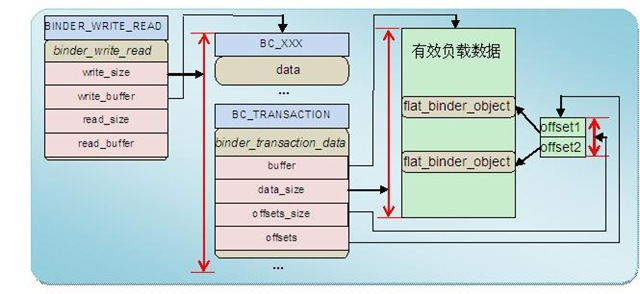
\includegraphics[scale=0.66]{binderproto.jpg}

\caption{ BINDER_WRITE_READ数据包结构\label{fig:BinderData}}
\end{minipage}

\subsection{flat_binder_object}
Binder可以塞在数据包的有效数据中越进程边界从一个进程传递给另一个进程,这些传输
中的Binder用结构flat_binder_object\ref{fig:BinderData}表示,如下表所示: 

\begin{lstlisting}[caption={flat\_binder\_object}, label=flatbinderobject]
/*
 * This is the flattened representation of a Binder object for transfer
 * between processes.  The 'offsets' supplied as part of a binder transaction
 * contains offsets into the data where these structures occur.  The Binder
 * driver takes care of re-writing the structure type and data as it moves
 * between processes.
 */
struct flat_binder_object {
	/* 8 bytes for large_flat_header. */
	unsigned long		type;
	unsigned long		flags;

	/* 8 bytes of data. */
	union {
		void		*binder;	/* local object */
		signed long	handle;		/* remote object */
	};

	/* extra data associated with local object */
	void			*cookie;
};

\end{lstlisting}
前面说过 \binder
有两种存在方式,所以用户程序必须区分这两种存在,但是对于应用程序来说,由于使用
了对象的公共接口,高层用户不必知道到底是哪一种 \binder ,这个工作是由 c++ 的
Binder 库完成的。对于 Binder 库来说,他必须区分是哪种 \binder ,他与驱动的沟通
便是用的这个结构体。这个结构体是驱动和 Binder 库共用的,在 binder.h 里定义。
%\setdescription{labelsep=3pt}
\begin{description}
    \item [type]
        
        type 表示 \binder 的类型,一共5种:
        %\begin{lstlisting}[language=,multicols=2,label=bindertype, title=Binder Type, numbers=none]
        %\end{lstlisting}
         BINDER_TYPE_BINDER 和 BINDER_TYPE_WEAK_BINDER 都是本地 \binder,对应于
        binder_node,BINDER_TYPE_HANDLE 和 BINDER_TYPE_WEAK_HANDLE 都是远程 \binder (即引用),对应于 binder_desc 。至于
        WEAK 不 WEAK 跟指针的引用强度有关。\binder
        除了是个跨进程的指针之外,还能当做跨进程文件描述符用,BINDER_TYPE_FD
        类型就是干这个的。
    \item [binder/handle]
        
        联合体 binder/handle 就对应于 binder_node 的 ptr 或者 binder_desc 的
        desc,取决于他是 BINDER 还是 HANDLE。
        当传递的是Binder实体时使用binder域,指向Binder实体在应用程序中的地址。
        当传递的是Binder引用时使用handle域,存放Binder在进程中的引用号。

    \item [cookie] 
        
        cookie在BINDER类型时就是binder_node的cookie,存放与该Binder有关的附加信息。
        在HANDLE时是null,没啥用。

    \item [flags]
        
            flags 的 7\~{}0 bits 是用来设置 binder_node 的线程优先级的,在
            binder 的实际应用中,远程进程的对 \binder 的操作请求会由\binder
            本地进程的一个线程完成,而这个优先级就是用来设置该线程处理这个
            \binder 事物时的优先级。

            flags 的 8th bits 是用来表示这个binder是否接受文件描述符的,不支持
            文件描述符的 \binder 是没法用 BINDER_TYPE_FD 的。
\end{description}

这个结构体非常重要,用起来也很隐蔽。俗话说一个巴掌拍不响,如果没有这个结构体,光有驱动里的
binder_node 几个结构体,跨进程的指针也是不好实现的,因为无论 ptr 还是 desc
归根到底只是个 32 比特的数(假设是 32 位系统),
一个进程光靠这个数是没法区分这是本地还是远程 binder,而驱动光知道 proc
和一个数也是没法清楚用户程序要的是本地还是远程 \binder,需要 type
这个值才能分清楚是远程还是本地 \binder \footnote{其实我觉得也可以通过 debug_id
来标识,可惜慢了点}。虽然对于事物请求 (transaction)
,驱动和应用程序可以假定目标 \binder 指的远程 \binder
,但是想要在两个进程之间传递一个 \binder 就无法做到了,而这个正是 android 的
binder 头号程序 service manager 做的事情, android
各种服务程序和应用程序之间也是通过这种方式传递对象 binder
的。


正如前面所说,这个结构体主要是用来在进程间传递 \binder
而设计的,只会发生在进程间 transaction 时,transaction 数据里的 offsets 和
offsets_size 便是用来存放这个结构体的,当 transaction
发生时,驱动会修改这里面的数据,把请求方进程的 \binder 转换成 transaction
目标进程的里的 \binder,可能是远程到本地,本地到远程甚至是远程到远程 \binder
的转换。


驱动不仅仅只是完成 \binder 的转换和传递,必要时还得创建 binder_node 和
binder_ref,分两种情况。一个是
ioctl(BINDER_SET_CONTEXT_MGR),这个是某个进程(注:即 service manager
进程,比较特殊,这个 binder_node 不是对象,ptr 和 cookie 都为 0)把自己注册为
binder 的服务程序。而进程与 service manager
通信时,如果还没有 service manager 的远程 binder 时,便会创建一个binder_ref。

除了上面的特殊情况,binder_node 和 binder_ref
的创建只可能发生在前面提到的在进程间通过 transaction 传递 binder 时。当
transaction 传递一个本地 \binder 时,如果该 \binder
在驱动中并没有记录,驱动便调用 binder_new_node 为其创建一个 binder_node
。不论传递远程还是本地 \binder,如果该 \binder 在目标进程中没有记录,驱动调用
binder_get_ref_for_node 为目标进程创建一个 binder_ref。由于 binder 和c++的
binder 库使用了引用计数, binder的创建到此才刚上路,接下来是极其复杂的引用计数。

无论是Binder实体还是对实体的引用都从属与某个进程,所以该结构不能透明地在进程之
间传输,必须经过驱动翻译。例如当Server把Binder实体传递给Client时,在发送数据流
中,flat_binder_object中的type是BINDER_TYPE_BINDER,binder指向Server进程用户空
间地址。如果透传给接收端将毫无用处,驱动必须对数据流中的这个Binder做修改:将
type该成BINDER_TYPE_HANDLE;为这个Binder在接收进程中创建位于内核中的引用并将引
用号填入handle中。对于发生数据流中引用类型的Binder也要做同样转换。经过处理后接
收进程从数据流中取得的Binder引用才是有效的,才可以将其填入数据包
binder_transaction_data的target.handle域,向Binder实体发送请求。
下表总结了当flat_binder_object结构穿过驱动时驱动所做的操作:

\begin{longtable}{|p{0.3\textwidth}|p{0.35\textwidth}|p{0.35\textwidth}|}\hline
    Binder 类型( type 域) & 在发送方的操作 & 在接收方的操作 \\\hline
    BINDER_TYPE_BINDER \newline BINDER_TYPE_WEAK_BINDER &
    只有实体所在的进程能发送该类型的Binder。如果是第一次发送驱动将创建实体在内核中
    的节点,并保存binder,cookie,flag域。&
    如果是第一次接收该Binder则创建实体在内核中的引用;将handle域替换为新建的引用号
    ;将type域替换为BINDER_TYPE_(WEAK_)HANDLE \\\hline
    BINDER_TYPE_HANDLE \newline BINDER_TYPE_WEAK_HANDLE &
    获得Binder引用的进程都能发送该类型Binder。驱动根据handle域提供的引用号查找建立
    在内核的引用。如果找到说明引用号合法,否则拒绝该发送请求。 &
    如果收到的Binder实体位于接收进程中:将ptr域替换为保存在节点中的binder值;
    cookie替换为保存在节点中的cookie值;type替换为BINDER_TYPE_(WEAK_)BINDER。如果
    收到的Binder实体不在接收进程中:如果是第一次接收则创建实体在内核中的引用;将
    handle域替换为新建的引用号  \\\hline
    BINDER_TYPE_FD & 验证handle域中提供的打开文件号是否有效,无效则拒绝该发送请求
    。 & 在接收方创建新的打开文件号并将其与提供的打开文件描述结构绑定。\\\hline
\end{longtable}


文件形式的 Binder

除了通常意义上用来通信的Binder,还有一种特殊的Binder:文件Binder。这种Binder的
基本思想是:将文件看成Binder实体,进程打开的文件号看成Binder的引用。一个进程可
以将它打开文件的文件号传递给另一个进程,从而另一个进程也打开了同一个文件,就象
Binder的引用在进程之间传递一样。

一个进程打开一个文件,就获得与该文件绑定的打开文件号。从Binder的角度,linux在
内核创建的打开文件描述结构struct
file是Binder的实体,打开文件号是该进程对该实体的引用。既然是Binder那么就可以在
进程之间传递,故也可以用flat_binder_object结构将文件Binder通过数据包发送至其它
进程,只是结构中type域的值为BINDER_TYPE_FD,表明该Binder是文件Binder。而结构中
的handle域则存放文件在发送方进程中的打开文件号。我们知道打开文件号是个局限于某
个进程的值,一旦跨进程就没有意义了。这一点和Binder实体用户指针或Binder引用号是
一样的,若要跨进程同样需要驱动做转换。驱动在接收Binder的进程空间创建一个新的打
开文件号,将它与已有的打开文件描述结构struct
file勾连上,从此该Binder实体又多了一个引用。新建的打开文件号覆盖
flat_binder_object中原来的文件号交给接收进程。接收进程利用它可以执行read(),
write()等文件操作。

传个文件为啥要这么麻烦,直接将文件名用Binder传过去,接收方用open()打开不就行了
吗?其实这还是有区别的。首先对同一个打开文件共享的层次不同:使用文件Binder打开
的文件共享linux VFS中的struct file,struct dentry,struct inode结构,这意味着
一个进程使用 read()/write()/seek() 改变了文件指针,另一个进程的文件指针也会改
变;而如果两个进程分别使用同一文件名打开文件则有各自的struct file
结构,从而各自独立维护文件指针,互不干扰。其次是一些特殊设备文件要求在
struct file 一级共享才能使用,例如 android 的另一个驱动 ashmem,它和 Binder 一样也是misc设
备,用以实现进程间的共享内存。一个进程打开的ashmem文件只有通过文件Binder发送到
另一个进程才能实现内存共享,这大大提高了内存共享的安全性,道理和Binder增强了
IPC的安全性是一样的。

\section{Binder Driver}

\subsection{重要的数据结构}
\subsubsection{binder_proc 结构体}
用来表示进程的
\begin{lstlisting}[language=KC, multicols=2]
struct binder_proc {
    struct hlist_node proc_node;
    struct rb_root threads;
    struct rb_root nodes;
    struct rb_root refs_by_desc;
    struct rb_root refs_by_node;
    int pid;
    struct vm_area_struct *vma;
    struct task_struct *tsk;
    struct files_struct *files;
    struct hlist_node deferred_work_node;
    int deferred_work;
    void *buffer;
    ptrdiff_t user_buffer_offset;
    struct list_head buffers;
    struct rb_root free_buffers;
    struct rb_root allocated_buffers;
    size_t free_async_space;
    struct page **pages;
    size_t buffer_size;
    uint32_t buffer_free;
    struct list_head todo;
    wait_queue_head_t wait;
    struct binder_stats stats;
    struct list_head delivered_death;
    int max_threads;
    int requested_threads;
    int requested_threads_started;
    int ready_threads;
    long default_priority;
    struct dentry *debugfs_entry;
};
\end{lstlisting}
首先,这个结构体得能表示一个进程以及记录一个进程的资源,成员变量 pid, tsk,
files 就是用来干这些的,另外还有 threads 和 page, buffer 之类的成员也是用来表
示进程资源的,不过他们还有其他用途,以后再详细写。\\
其次,既然进程在两种存在方式里都是第一维,那么通过它,我们应该能够得到进程所有
的 binder(本地的以及远程的),他的 nodes, refs_by_desc, refs_by_node 就是用来
实现这个的,这三个都是红黑树根节点,具体的意义下面会详细解释。\\
debugfs_entry对应于上篇文章里的proc文件/proc/binder/proc/\various{pid}。
还有一些变量与 work 相关,以后再写。

\subsubsection{binder_node}
struct binder_node 是 Binder 实体在驱动中的表述. 驱动中的Binder实体也叫‘节点’,隶属于提供实体的进程,由struct binder_node结构来表示:

\begin{lstlisting}[language=C,multicols=2]
struct binder_node {
    int debug_id;
    struct binder_work work;
    union {
        struct rb_node rb_node;
        struct hlist_node dead_node;
    };
    struct binder_proc *proc;
    struct hlist_head refs;
    int internal_strong_refs;
    int local_weak_refs;
    int local_strong_refs;
    void __user *ptr;
    void __user *cookie;
    unsigned has_strong_ref:1;
    unsigned pending_strong_ref:1;
    unsigned has_weak_ref:1;
    unsigned pending_weak_ref:1;
    unsigned has_async_transaction:1;
    unsigned accept_fds:1;
    unsigned min_priority:8;
    struct list_head async_todo;
};
\end{lstlisting}
\tabcaption{结构成员解析}
\begin{longtable}{|p{0.3\textwidth}|p{0.7\textwidth}|}\hline
    work& 当本节点引用计数发生改变,需要通知所属进程时,通过该成员挂入所属进程的to-do队列里,唤醒所属进程执行Binder实体引用计数的修改。\\\hline
    rb_node\newline dead_node & 每个进程都维护一棵红黑树,以Binder实体在用户空间的指针,
    即本结构的ptr成员为索引存放该进程所有的Binder实体。这样驱动可以根据Binder
    实体在用户空间的指针很快找到其位于内核的节点。rb_node用于将本节点链入该红黑树中。
    销毁节点时须将rb_node从红黑树中摘除,但如果本节点还有引用没有切断,就用
    dead_node将节点隔离到另一个链表中,直到通知所有进程切断与该节点的引用后,该节
    点才可能被销毁。 \\\hline
    proc & 本成员指向节点所属的进程,即提供该节点的进程。\\\hline
    refs & 本成员是队列头,所有指向本节点的引用都链接在该队列里。这些引用可能隶属于不
    同的进程。通过该队列可以遍历指向该节点的所有引用。\\\hline
    internal_strong_refs & 用以实现强指针的计数器:产生一个指向本节点的强引用
    该计数就会加1 \\\hline
     local_weak_refs & 驱动为传输中的Binder设置的弱引用计数。如果一个Binder打包
     在数据包中从一个进程发送到另一个进程,驱动会为该Binder增加引用计数,
     直到接收进程通过BC_FREE_BUFFER通知驱动释放该数据包的数据区为止。\\\hline
      local_strong_refs & 驱动为传输中的Binder设置的强引用计数。同上。\\\hline
      ptr & 指向用户空间Binder实体的指针,来自于flat_binder_object的binder成员
      \\\hline
      cookie & 指向用户空间的附加指针,来自于flat_binder_object的cookie成员
      \\\hline
      has_strong_ref\newline pending_strong_ref \newline has_weak_ref \newline
      pending_weak_ref & 这一组标志用于控制驱动与Binder实体所在进程交互式修改
      引用计数 \\\hline
      has_async_transaction & 该成员表明该节点在to-do队列中有异步交互尚未完成。
      驱动将所有发送往接收端的数据包暂存在接收进程或线程开辟的to-do队列里。
      对于异步交互,驱动做了适当流控:如果to-do队列里有异步交互尚待处理则该成
      员置1,这将导致新到的异步交互存放在本结构成员 – asynch_todo队列中,而不
      直接送到to-do队列里。目的是为同步交互让路,避免长时间阻塞发送端。
      \\\hline
      accept_fds & 表明节点是否同意接受文件方式的Binder,来自flat_binder_object
      中flags成员的FLAT_BINDER_FLAG_ACCEPTS_FDS位。由于接收文件Binder会为进程自动
      打开一个文件,占用有限的文件描述符,节点可以设置该位拒绝这种行为。
      \\\hline
      min_priority & 设置处理Binder请求的线程的最低优先级。发送线程将数据提交给接收线程处理时,
      驱动会将发送线程的优先级也赋予接收线程,使得数据即使跨了进程也能以同样
      优先级得到处理。不过如果发送线程优先级过低,接收线程将以预设的最小值运行。
      该域的值来自于flat_binder_object中flags成员。\\\hline
      async_todo & 异步交互等待队列;用于分流发往本节点的异步交互包 \\\hline
  \end{longtable}
    每个进程都有一棵红黑树用于存放创建好的节点,以Binder
    在用户空间的指针作为索引。每当在传输数据中侦测到一个
    代表Binder实体的flat_binder_object,先以该结构的
    binder指针为索引搜索红黑树;如果没找到就创建一个新
    节点添加到树中。由于对于同一个进程来说内存地址是唯一
    的,所以不会重复建设造成混乱。


他是用来表示本地 binder 的,通过这个结构体能找到 binder 所在进程,也能找到
binder 在这个进程里的指针。 proc 记录了所在进程, cookie 和 ptr 记录了他在所在
进程中的指针,其实 cookie 才是真正的指针,而 ptr 是应用层为了引用计数弄出来的
一个东西,对于驱动来说,两者有些重复。而 debug_id 则是 binder_node 在驱动里的
全局 id ,前面一篇文章里的/proc/binder/下的信息里就会大量使用这个 debug_id ,
有了它就知道指的是哪个 binder_node 了,除了 binder_node ,还有几类信息也有
debug_id ,这几类的 debug_id 在驱动里从1开始统一排的。其实也可以用 debug_id 这
个一维的索引来表示 binder ,不过效率会比红黑树低,所以它只能当做 debug 信息用
。这个结构体还有一堆 ref 相关的成员,用于维护引用计数,以后再写。


 binder_proc 里的 nodes 这棵树便是用来遍历一个进程的本地 binder 即 binder_node
 的,为了快速查找, nodes 是颗二叉搜索数, key 是 binder_node 的 ptr 。按照
 linux 的惯例, binder_node 里需要有个成员,才能把它加到树或者列表里,而这个成
 员便是 rb_node ,通过 rb_node ,可以把 binder_node 与 binder_proc 的 nodes 关
 联,从而实现对一个进程的本地 binder 的管理。另外,这个 rb_node 是一个 union
 ,另一个名字叫做 dead_node ,这个身份是为了处理死亡的 binder 的,当一个进程结
 束时,他的本地 binder 自然也就挂了, binder_node 也就没必要存在了,但是由于别
 的进程可能正在使用这个 binder ,所以一时半会,驱动还没法直接移除这个
 binder_node ,不过由于进程挂了,驱动没法继续把这个 binder_node 挂靠在对应的
 binder_proc 下,只好把它挂靠在 binder_dead_nodes 下面。不过,这个
 binder_dead_nodes 其实也没啥意义,也就是打印/proc/binder/state时用了一下,看
 看当前有多少已经死亡但没移除的 binder_node 。驱动里真正移除一个死亡的
 binder_node 是靠引用计数的机制来完成的。

 \subsubsection{binder_ref}
 binder在远程进程中的表示, 也就是 Binder 引用在驱动中的表述.
     \begin{lstlisting}[language=KC, multicols=2]
struct binder_ref {
	/* Lookups needed: */
	/*   node + proc => ref (transaction) */
	/*   desc + proc => ref (transaction, inc/dec ref) */
	/*   node => refs + procs (proc exit) */
	int debug_id;
	struct rb_node rb_node_desc;
	struct rb_node rb_node_node;
	struct hlist_node node_entry;
	struct binder_proc *proc;
	struct binder_node *node;
	uint32_t desc;
	int strong;
	int weak;
	struct binder_ref_death *death;
};
\end{lstlisting}
  和实体一样,Binder的引用也是驱动根据传输数据中的flat_binder_object创建的,隶属于获得该引用的进程,用struct binder_ref结构体表示:

\tabcaption{Binder引用描述结构:binder_ref}
\begin{longtable}{|p{0.3\textwidth}|p{0.7\textwidth}|}\hline
    rb_node_desc & 每个进程有一棵红黑树,进程所有引用以引用号(即本结构的desc域)
    为索引添入该树中。本成员用做链接到该树的一个节点。\\\hline
    rb_node_node & 每个进程又有一棵红黑树,进程所有引用以节点实体在驱动中的
    内存地址(即本结构的node域)为所引添入该树中。本成员用做链接到该树的一个节
    点。\\\hline
    node_entry & 该域将本引用做为节点链入所指向的Binder实体结构binder_node中的
    refs队列 \\\hline
    proc & 本引用所属的进程 \\\hline 
    node & 本引用所指向的节点(Binder实体)\\\hline
    desc & 本结构的引用号 \\\hline
    strong & 强引用计数 \\\hline
    weak & 弱引用计数 \\\hline
    death & 应用程序向驱动发送BC_REQUEST_DEATH_NOTIFICATION或
    BC_CLEAR_DEATH_NOTIFICATION命令从而当Binder实体销毁时能够
    收到来自驱动的提醒。该域不为空表明用户订阅了对应实体销毁的‘噩耗’。\\\hline
\end{longtable}

就象一个对象有很多指针一样,同一个Binder实体可能有很多引用,不同的是这些引用可能分布在不同的进程中。和实体一样,每个进程使用红黑树存放所有正在使用的引用。不同的是Binder的引用可以通过两个键值索引:

· 对应实体在内核中的地址。注意这里指的是驱动创建于内核中的binder_node结构的地址,而不是Binder实体在用户进程中的地址。实体在内核中的地址是唯一的,用做索引不会产生二义性;但实体可能来自不同用户进程,而实体在不同用户进程中的地址可能重合,不能用来做索引。驱动利用该红黑树在一个进程中快速查找某个Binder实体所对应的引用(一个实体在一个进程中只建立一个引用)。

· 引用号。引用号是驱动为引用分配的一个32位标识,在一个进程内是唯一的,而在不同进程中可能会有同样的值,这和进程的打开文件号很类似。引用号将返回给应用程序,可以看作Binder引用在用户进程中的句柄。除了0号引用在所有进程里都固定保留给SMgr,其它值由驱动动态分配。向Binder发送数据包时,应用程序将引用号填入binder_transaction_data结构的target.handle域中表明该数据包的目的Binder。驱动根据该引用号在红黑树中找到引用的binder_ref结构,进而通过其node域知道目标Binder实体所在的进程及其它相关信息,实现数据包的路由。


与 binder_node 类似,拥有 proc 和 debug_id 。然后便是重要的 desc ,即前面提到
的0开始递增的数字,这个数字和 proc 也就能唯一确定一个远程的 binder ,也就是跨
进程 binder 在另一个进程里的表示,而 node 指向这个 binder 的本地进程表示
binder_node 。由于一个本地 binder 可以被多个进程使用,于是一个 binder_node 可
能有多个 binder_ref 来对应,所以 binder_node 中有个 refs 的链表用来记录他的远
程表示,而 node_entry 就是用于这个链表的,这个没用红黑树,因为这个表一般比较小
,而且用不着搜索。 rb_node_desc 用于 binder_proc 的 refs_by_desc ,
rb_node_node 用于 binder_proc 的 refs_by_node ,这两都是二叉搜索树,前一个 key
是 desc ,后一个 key 是 node 。如果已知 binder 的远程表示 proc + desc ,就可以
用 refs_by_desc 查找,如果知道本地表示则用 refs_by_node 查找,看看某个远程
proc 是否已经具备该 binder_node 的远程表示。 strong 和 weak 两个变量是用于引用
的, death 则是用于死亡通知的,以后再写。

\subsubsection{数据结构的关系}
总结一下, binder 是跨进程的指针,有两种形式,一是在本地进程里,他就是个进程指
针,驱动中记为 binder_node ,其中 proc 为它的本地进程,ptr/cookie 为进程里的指
针,另一种是在远程进程里,他就是个从0开始增加的数(按该进程中远程 binder 出场
顺序记录),驱动里记为 binder_desc ,其中 proc 为远程进程, desc 为序号。驱动
中维护远程 binder 和本地 binder 的转换,包括远程(proc, desc)与本地(proc,
ptr)的互相转换,也包括远程(proc, desc)和另一个远程(proc,
desc)的互相转换,当然也支持本地到本地的转换(这种情况就是完全相同的一个东西)
,不过这种转换驱动里是不会发生的,上层的c++的 binder 库中已经识别了 binder 是
不是本地的,本地的 binder 自行就处理了,不需要经过驱动这层额外开销。


下面列几个相关的函数,以下省略struct关键字。
\begin{itemize}
    \item binder_node* binder_get_node(binder_proc *proc, void __user *ptr)

        给定ptr(binder_node中的ptr)和进程proc,在proc的nodes树中查找并获取binder_node
        结构,如果这个proc的这个指针在驱动里还没有建立本地binder,则返回null。

    \item binder_node* binder_new_node(binder_proc *proc, void __user *ptr, void __user *cookie)

        给定ptr和cookie以及进程proc,在驱动中创建该指针的本地binder项,并添加到proc的nodes树中。

    \item binder_ref *binder_get_ref(binder_proc *proc, uint32_t desc)

        给定desc和proc,获取远程binder的表示binder_desc,如果没有则返回null。

    \item binder_ref *binder_get_ref_for_node(binder_proc *proc, binder_node *node)

        给定proc和node,获取某个本地binder在该proc进程里的远程表示,如果该本地binder在
        该proc中还没有建立远程表示,则创建它并返回。此函数会用到并可能更新proc的
        refs_by_desc, refs_by_node树以及node的refs链表。

    \item binder_delete_ref(binder_ref *ref)

        删除给定的远程binder。并不存在binder_delete_node函数,node的删除是在node的引用
        计数减到0时发生的,被整合到了binder_dec_node函数。
\end{itemize}



\subsection{线程池}
\subsubsection{Binder 下的进程}
首先说一下进程,即 Linux 进程。驱动会使用上篇提到的 binder_proc
记录进程信息。每个要使用 Binder 驱动的进程都会在使用驱动前 open binder
驱动(废话…),驱动在 open 的时候会创建该结构体,初始化一些信息,
并把该结构体的指针记录到文件结构体的 private_data , 以后的驱动操作就能通过文件结构体获取该进程信息。

前面说过,进程是有自己独立的内存空间的,所以 Binder
这个东西是基于进程的,而不是线程,因为同一进程的不同线程是共用一个内存空间,没必要把
Binder 细分到线程,而且也不适合后面要说的线程池。因此驱动里都是以 binder_proc
为单元来分配和记录资源的,驱动会给每个进程创建一个 /proc/binder/proc/\various{pid}
文件,用来展示进程相关的 binder 信息,而进程的 binder 清理工作则是通过标记量
deferred_work 以及链表 deferred_work_node 实现的。至于 transaction
需要的内存空间则是通过一系列名字包含 buffer 和 page
的成员变量完成的,这个以后再写。


最重要的是,上一篇说的远程和本地 \binder 都是在 binder_proc
中有记录的,用的便是 proc_node, refs_by_desc, refs_by_node
三棵树。还有一棵重要的树,叫做 threads , 这个是用来记录进程中与 binder
有一腿的线程的,与线程相关的还有各种含 thread 的变量以及 todo,wait 和
default_priority 。 至于 delivered_death 则是用于死亡通知的,而 stats 是用于统计
binder 信息的, /proc/binder/stats 和 /proc/binder/proc/\various{pid} 能查到相应信息。

\subsubsection{Binder 下的线程}
Linux 的线程是轻量级的进程。 Binder 记录线程的数据结构是结构体 binder_thread
\begin{lstlisting}
struct binder_thread {
	struct binder_proc *proc;
	struct rb_node rb_node;
	int pid;
	int looper;
	struct binder_transaction *transaction_stack;
	struct list_head todo;
	uint32_t return_error; /* Write failed, return error code in read buf */
	uint32_t return_error2; /* Write failed, return error code in read */
		/* buffer. Used when sending a reply to a dead process that */
		/* we are also waiting on */
	wait_queue_head_t wait;
	struct binder_stats stats;
};
\end{lstlisting}

 proc 用来记录该线程所属进程的 binder_proc 结构体, pid 记录线程的 id , stats
同 proc 的,用于统计线程的 binder 信息, return_error 和 return_error2 用来记录
ioctl 的一些错误信息, transaction_stack 用于 transaction , looper
记录线程的状态,与后面的线程池相关。 wait 和 todo 则跟线程的工作相关。 

 rb_node 用来关联 binder_proc 的 threads 树,这也是一棵二叉搜索树, key
很显然便是线程的 pid 。有一个很重要的函数跟这棵树相关:
\begin{lstlisting}
binder_thread *binder_get_thread(binder_proc *proc)
\end{lstlisting}

任何一个线程执行 binder 驱动的 poll 和 ioctl 操作时,驱动都会从文件结构体获取
binder_proc 信息,然后尝试从这个进程信息里获取当前线程的信息,如果没找到,则为当前线程创建一个
binder_thread ,并记录到进程的 threads 中。所以,进程的 threads
只是记录了那些跟 binder 有一腿的线程的,而不会记录进程的所有线程。

\subsubsection{进程池}
写它之前,先简单的提一下 ioctl(BINDER _WRITE_READ) 。 这个 ioctl 有两步,第一
步是 write ,会传给驱动一些以 BC_ 开头的命令,让驱动去执行,一次可以传多个命令
。第二步是 read,会从驱动获取一些以 BR_ 开头的回复,也可能是多个,上层 binder
库可以根据这些回复做相应的操作, read 这一步有可能阻塞当前线程,直到驱动给他回
复并唤醒它。

所谓的线程池跟平时说的线程区别并不大, 进程会产生一些线程, 让他们做无限循环,
在循环里等待, 直到外界有工作传来, 该线程便被唤醒, 待到该线程干完活之后,
又继续循环, 再次进入等待状态,直到下一个工作来临。 不同的是,
传统的线程池的工作是本地进程里的某个不加入线程池的线程给的, 而 android
的线程池等待的工作则是由别的进程里的线程给的。这个工作由别的进程里的线程通过
BINDER_WRITE_READ 的 write 步骤提交给驱动,线程池中的线程则一直在循环做着
BINDER_WRITE_READ ,他们的 read 步骤会阻塞,直到驱动把别的线程通过 write
写过来的工作传给他们,线程池中的线程的 read 得以返回,便根据得到的 BR
进行相应的操作,之后再次 BINDER_WRITE_READ ,通过 write 把结果传回驱动,
然后线程又可能再次 BINDER_WRITE_READ 阻塞在 read 阶段等待新的工作。

驱动除了转交别的进程的工作,也可能自己产生工作给线程池做,同样是在线程池的 read
阶段返回给线程池。这一类包括一堆引用计数的工作,以及接下来要写的 LOOPER 工作。

\subsubsection{线程池的循环}\label{protocol:threadpool}
所谓的 LOOPER 就是线程池的无限循环,先来看看 LOOPER 相关的枚举量:
\begin{lstlisting}[multicols=2,caption=Binder Looper state]
enum {
    BINDER_LOOPER_STATE_REGISTERED = 0x01,
    BINDER_LOOPER_STATE_ENTERED = 0x02,
    BINDER_LOOPER_STATE_EXITED = 0x04,
    BINDER_LOOPER_STATE_INVALID = 0x08,
    BINDER_LOOPER_STATE_WAITING = 0x10,
    BINDER_LOOPER_STATE_NEED_RETURN = 0x20
};
\end{lstlisting}

这些标记(以下枚举量省略前缀 BINDER_LOOPER_STATE_ )会用于 proc_thread 的
looper 变量,用来表明线程的状态,下面会一一提到。


前面说的 work\marginpar{翻译成工作感觉太土了,不翻了}分为两类,一类是给指定线程的,叫
做线程 work,一类是给线程池的,叫做进程(线程池) work,这一类可能被线程池中任
意一个线程通过 read获取,而前者只会给指定线程获取。如果一个线程想加入线程池,
获取进程 work时,必须先告知驱动,需要通过 write 发送 BC_ENTER_LOOPER 或者
BC_REGISTER_LOOPER命令给驱动以表明自己进入了线程池循环,可以接受进程 work,驱
动会根据命令设置线程的 looper 的 ENTERED 或者 REGISTERED标志位。而一个线程如果
要退出线程池,需要发送 BC_EXIT_LOOPER 给驱动,此时 looper的 EXITED
标记被设置。一个线程(不一定加入了线程池)如果没有事情可做,在 read阶段阻塞时
, WAITING 标记被设置。


而 NEED_RETURN 状态则是所有线程的初始状态,这个状态如果被设置,线程不管有没有
work 要做, read 都将立刻返回,而这个标记在每次 ioctl后都被清零,就是说这个标
记正常情况只在第一次 ioctl时起作用,而几乎所有的线程的第一次 ioctl 都是 write
命令 BC_ENTER_LOOPER 或者BC_REGISTER_LOOPER 把自己加入线程池,所以不管线程池有
没有 work可做,这些线程在把自己注册到线程池后都会返回,这样用户程序才好得知线
程是否成功加入线程池。

有一个例外,任何一个进程用于 open 驱动的那个线程,一般是进程的主线程, binder
库中,这个线程在 open 驱动之后会进行 ioctl(BINDER_VERSION) 用来检测驱动版本,
便产生了副作用,此 ioctl 清除了主线程的 NEED_RETURN 标记,导致主线程在 ENTER_LOOPER
会被阻塞。于是有一个有趣的现象,应用程序里的主线程如果调用 joinThreadPool ,
BC_ENTER_LOOPER 时不会立刻返回,也就不会生成一个新的线程,而程序里用
startThreadPool 新起的线程在 BC_ENTER_LOOPER 后会返回,而且几乎肯定会再生成
一个新的线程。至于为啥会生成一个新的线程,后面写 BC_ENTER_LOOPER 和
 BC_REGISTER_LOOPER 的区别时会写到,那里也将涉及到最后一个状态 INVALID 。

关于 NEED_RETURN 还有一个非正常情况,那就是文件操作中的 flush , flush情况下会
设置所有线程的 NEED_RETURN 标记并唤醒 WAITING中的线程,这样所有的线程的 read
都会得到返回。


BC_ENTER_LOOPER 和 BC_REGISTER_LOOPER 都是用来将线程注册到驱动,以便他们
能够获取进程 work 。前者适用于应用程序自己主动产生的线程,比如主线程以及
startThreadPool 产生的第一个线程。

任何一个线程在read阶段返回时,会检查进程的ready_threads,这个变量表示当前进程
有多少个线程正在等待进程work,这类线程必然处于WAITING状态(反过来不一定成立
\^{}-\^{})。如果当前没有线程等待进程work,驱动在read的返回BR队列最前面加上一个
BR_SPAWN_LOOPER通知该线程,线程池已经没有可用于处理进程work的线程了,你得赶紧
给我产生一个新的,线程在read返回之后便会根据该BR创建一个新的线程,并让它
BC_REGISTER_LOOPER加入线程池并待命,然后自己才去处理这次read到的真正work,这样
可以缩短线程池的真空期。

这里有点小优化,如果驱动已经要求某个线程生成一个新的线程,在这个线程还没加入线
程池前,驱动不会在别的线程read返回时再次要求生成新线程,这样可以避免要求进程生
成过多的线程。这件事情是通过进程的requested_threads变量实现的,在read返回
BR_SPAWN_LOOPER时,此变量被增加,在新的线程BC_REGISTER_LOOPER成功时此变量被减
小,用来表明生成线程的工作已经完成,而通过这种方式生成的线程数会被记录到进程的
reqeusted_threads_started,这种方式生成的线程数不能超过进程的max_threads,此数
通过ioctl(BINDER_SET_MAX_THREADS)设置,binder库中设置为15。注意,这个MAX并不约
束进程的线程数,也不约束线程池中的线程数,仅仅约束在驱动要求下生成的线程数,即
通过BC_REGISTER_LOOPER加入线程池的线程数。

如果到了MAX后,线程池中的线程还不够响应远程请求时,用户进程可以自行生成新的线
程并用BC_ENTER_LOOPER注册到线程池用来提供服务。不过一般没必要这么做,线程多了
并不见得能改善服务速度,还不如让请求等待着,直到线程池已有的线程完成手头工作再
去响应新的请求。

最后一个状态INVALID便是与这两种BC相关,如果一个ENTERED的线程发起
BC_REGISTER_LOOPER或者REGISTERD的线程发起BC_ENTER_LOOPER,都会被标记为INVALID
状态。而一个线程发起BC_REGISTER_LOOPER时,驱动会检查requested_threads,如果它
发现自己并没有要求哪个线程生成新的线程并让其BC_REGISTER_LOOPER,也会将该线程标
记为INVALID。


\subsection{ work}
work分两种,进程work和线程work,分别记录在binder_proc和binder_thread的todo列表
里。线程在ioctl(BINDER_WRITE_READ)的read阶段如果任何一种work以及NEED_RETURN都
没有的话,线程便会阻塞,根据线程的情况可能加入到进程的wait队列,这个wait是
exclusive的,因为进程的一个work只需要唤醒一个线程来做即可,也有可能加入到线程
的wait队列(这个队列最多也就线程本身),这些写BINDER_WRITE_READ的时候再详述。

work本身用binder_work表示,如下:
\begin{lstlisting}
struct binder_work {
struct list_head entry;
enum {
BINDER_WORK_TRANSACTION = 1,
BINDER_WORK_TRANSACTION_COMPLETE,
BINDER_WORK_NODE,
BINDER_WORK_DEAD_BINDER,
BINDER_WORK_DEAD_BINDER_AND_CLEAR,
BINDER_WORK_CLEAR_DEATH_NOTIFICATION,
} type;
};
\end{lstlisting}
entry是用来把work加入到相应todo里的。而type(以下略去前缀BINDER_WORK_)则是work的性质。

TRANSACTION类型的work就是前面多次提到的transaction,android里进程之间普通的请
求就是这个东西,这里先简单说下流程,以后再详写实现。

通常,一个线程需要另一个进程的binder进行服务时,它会write
BC_TRANSCATION向某个binder来发起transaction,驱动会创建一个TRANSACTION类型的
work,并把它加到binder所在进程work里,然后唤醒线程池中的一个线程,让他去完成这
个请求。binder完成任务时,所在的线程会write
BC_REPLY发回transaction完成的结果,此时驱动也会创建一个TRANSACTION类型的work,
并把它加到transaction发起者的线程work里,然后唤醒发起线程。这一来一去有个很大
不同之处便是接受者,发起transaction时面对是整个线程池,所以work会被加到目标进
程的work里,而transaction回复时是知道发起者线程的,所以是加到线程work中。

在上述过程中,BC_TRANSACTION和BC_REPLY的write完成时,驱动会立刻往写入命令的线
程work中增加一个TRANSACTION_COMPLETE类型的work,以便让线程再接下来的read阶段能
够立刻返回。这点跟我最开始想象的不同,刚开始接触binder时没看驱动,一直以为线程
发出BC_TRANSACTION后会阻塞在read阶段,直到收到目标binder发回的BC_REPLY才返回。
看了驱动才知道,这个操作是会立刻返回BR_TRANSACTION_COMPLETE的,但是binder库中
的transact在发出BC_TRANSACTION并收到这个BR后,会立刻再次进行
iocl(BINDER_WRITE_READ)进入等待状态,直到远端的binder实际完成transaction,所以
看起来线程就像是在发出transaction后便阻塞了。

NODE类型的work是用于引用计数的,当binder_node的引用计数发生某些变化时,驱动就
会往进程或者线程的work里添加这个binder_node的work,还记得binder_node里的work成
员变量么。写引用计数的时候再详细写这个。

DEAD_BINDER,DEAD_BINDER_AND_CLEAR,CLEAR_DEATH_NOTIFICATION这三种类型是用于死
亡通知的,有空再写。最后要提一点,驱动在处理各种work时,会考虑当前线程LOOPER状
态,如果没有ENTERED或者REGISTERED的,便一定会把work添加到进程work里,否则很可
能加到当前线程的work里,这个得看实际情况了。


总结一下binder和进程,线程,线程池的关系。binder本质是个跨进程的指针,只需要跟
进程挂钩,所以它可以被进程的任意一个线程处理,于是android这种服务于其他进程的
线程池便有了存在的根基。android中一个本地binder一般就对应着一个服务,会有很多
请求者,所以用线程池来响应是比较合适的。各种LOOPER状态使得应用程序的线程池能够
很好的投影到驱动里,保持高度的一致性。而驱动要求线程spawn线程的机制与binder库
的无缝结合,使得高层用户不用关心线程池的容量,高层用户只需要知道线程池他不是一
个线程在战斗就行了,线程池搞不定时他会自己再生出一个线程来帮手的。而进程中的远
程binder一般却是活在特定线程中,他们是服务请求的发起者,所以无所谓用线程池来响
应请求,而且他们一般是由应用程序某个特定线程调度,用来完成特殊命令的,这样的线
程是不愿意让别的线程获取自己发出的请求的答复的,所以远程binder虽然是活在进程里
,但是他永远住在某个特定的线程,从不搬家。至于work的性质,添加和移除,则跟
transaction,引用以及死亡通知相关,以后再详写。


\subsection{Binder 接收线程管理}
Binder通信实际上是位于不同进程中的线程之间的通信。假如进程S是Server端,提供Binder实体,线程T1从Client进程C1中通过Binder的引用向进程S发送请求。S为了处理这个请求需要启动线程T2,而此时线程T1处于接收返回数据的等待状态。T2处理完请求就会将处理结果返回给T1,T1被唤醒得到处理结果。在这过程中,T2仿佛T1在进程S中的代理,代表T1执行远程任务,而给T1的感觉就是象穿越到S中执行一段代码又回到了C1。为了使这种穿越更加真实,驱动会将T1的一些属性赋给T2,特别是T1的优先级nice,这样T2会使用和T1类似的时间完成任务。很多资料会用‘线程迁移’来形容这种现象,容易让人产生误解。一来线程根本不可能在进程之间跳来跳去,二来T2除了和T1优先级一样,其它没有相同之处,包括身份,打开文件,栈大小,信号处理,私有数据等。

对于Server进程S,可能会有许多Client同时发起请求,为了提高效率往往开辟线程池并发处理收到的请求。怎样使用线程池实现并发处理呢?这和具体的IPC机制有关。拿socket举例,Server端的socket设置为侦听模式,有一个专门的线程使用该socket侦听来自Client的连接请求,即阻塞在accept()上。这个socket就象一只会生蛋的鸡,一旦收到来自Client的请求就会生一个蛋 – 创建新socket并从accept()返回。侦听线程从线程池中启动一个工作线程并将刚下的蛋交给该线程。后续业务处理就由该线程完成并通过这个单与Client实现交互。

可是对于Binder来说,既没有侦听模式也不会下蛋,怎样管理线程池呢?一种简单的做法是,不管三七二十一,先创建一堆线程,每个线程都用BINDER_WRITE_READ命令读Binder。这些线程会阻塞在驱动为该Binder设置的等待队列上,一旦有来自Client的数据驱动会从队列中唤醒一个线程来处理。这样做简单直观,省去了线程池,但一开始就创建一堆线程有点浪费资源。于是Binder协议引入了专门命令或消息帮助用户管理线程池,包括:

· INDER_SET_MAX_THREADS\\* 
· BC_REGISTER_LOOP     \\*
· BC_ENTER_LOOP        \\*
· BC_EXIT_LOOP         \\*
· BR_SPAWN_LOOPER      \\*

首先要管理线程池就要知道池子有多大,应用程序通过INDER_SET_MAX_THREADS告诉驱动最多可以创建几个线程。以后每个线程在创建,进入主循环,退出主循环时都要分别使用BC_REGISTER_LOOP,BC_ENTER_LOOP,BC_EXIT_LOOP告知驱动,以便驱动收集和记录当前线程池的状态。每当驱动接收完数据包返回读Binder的线程时,都要检查一下是不是已经没有闲置线程了。如果是,而且线程总数不会超出线程池最大线程数,就会在当前读出的数据包后面再追加一条BR_SPAWN_LOOPER消息,告诉用户线程即将不够用了,请再启动一些,否则下一个请求可能不能及时响应。新线程一启动又会通过BC_xxx_LOOP告知驱动更新状态。这样只要线程没有耗尽,总是有空闲线程在等待队列中随时待命,及时处理请求。

关于工作线程的启动,Binder驱动还做了一点小小的优化。当进程P1的线程T1向进程P2发送请求时,驱动会先查看一下线程T1是否也正在处理来自P2某个线程请求但尚未完成(没有发送回复)。这种情况通常发生在两个进程都有Binder实体并互相对发时请求时。假如驱动在进程P2中发现了这样的线程,比如说T2,就会要求T2来处理T1的这次请求。因为T2既然向T1发送了请求尚未得到返回包,说明T2肯定(或将会)阻塞在读取返回包的状态。这时候可以让T2顺便做点事情,总比等在那里闲着好。而且如果T2不是线程池中的线程还可以为线程池分担部分工作,减少线程池使用率。

\subsection{8 数据包接收队列与(线程)等待队列管理}
通常数据传输的接收端有两个队列:数据包接收队列和(线程)等待队列,用以缓解供需矛盾。当超市里的进货(数据包)太多,货物会堆积在仓库里;购物的人(线程)太多,会排队等待在收银台,道理是一样的。在驱动中,每个进程有一个全局的接收队列,也叫to-do队列,存放不是发往特定线程的数据包;相应地有一个全局等待队列,所有等待从全局接收队列里收数据的线程在该队列里排队。每个线程有自己私有的to-do队列,存放发送给该线程的数据包;相应的每个线程都有各自私有等待队列,专门用于本线程等待接收自己to-do队列里的数据。虽然名叫队列,其实线程私有等待队列中最多只有一个线程,即它自己。

由于发送时没有特别标记,驱动怎么判断哪些数据包该送入全局to-do队列,哪些数据包该送入特定线程的to-do队列呢?这里有两条规则。规则1:Client发给Server的请求数据包都提交到Server进程的全局to-do队列。不过有个特例,就是上节谈到的Binder对工作线程启动的优化。经过优化,来自T1的请求不是提交给P2的全局to-do队列,而是送入了T2的私有to-do队列。规则2:对同步请求的返回数据包(由BC_REPLY发送的包)都发送到发起请求的线程的私有to-do队列中。如上面的例子,如果进程P1的线程T1发给进程P2的线程T2的是同步请求,那么T2返回的数据包将送进T1的私有to-do队列而不会提交到P1的全局to-do队列。

数据包进入接收队列的潜规则也就决定了线程进入等待队列的潜规则,即一个线程只要不接收返回数据包则应该在全局等待队列中等待新任务,否则就应该在其私有等待队列中等待Server的返回数据。还是上面的例子,T1在向T2发送同步请求后就必须等待在它私有等待队列中,而不是在P1的全局等待队列中排队,否则将得不到T2的返回的数据包。

这些潜规则是驱动对Binder通信双方施加的限制条件,体现在应用程序上就是同步请求交互过程中的线程一致性:1) Client端,等待返回包的线程必须是发送请求的线程,而不能由一个线程发送请求包,另一个线程等待接收包,否则将收不到返回包;2) Server端,发送对应返回数据包的线程必须是收到请求数据包的线程,否则返回的数据包将无法送交发送请求的线程。这是因为返回数据包的目的Binder不是用户指定的,而是驱动记录在收到请求数据包的线程里,如果发送返回包的线程不是收到请求包的线程驱动将无从知晓返回包将送往何处。

接下来探讨一下Binder驱动是如何递交同步交互和异步交互的。我们知道,同步交互和异步交互的区别是同步交互的请求端(client)在发出请求数据包后须要等待应答端(Server)的返回数据包,而异步交互的发送端发出请求数据包后交互即结束。对于这两种交互的请求数据包,驱动可以不管三七二十一,统统丢到接收端的to-do队列中一个个处理。但驱动并没有这样做,而是对异步交互做了限流,令其为同步交互让路,具体做法是:对于某个Binder实体,只要有一个异步交互没有处理完毕,例如正在被某个线程处理或还在任意一条to-do队列中排队,那么接下来发给该实体的异步交互包将不再投递到to-do队列中,而是阻塞在驱动为该实体开辟的异步交互接收队列(Binder节点的async_todo域)中,但这期间同步交互依旧不受限制直接进入to-do队列获得处理。一直到该异步交互处理完毕下一个异步交互方可以脱离异步交互队列进入to-do队列中。之所以要这么做是因为同步交互的请求端需要等待返回包,必须迅速处理完毕以免影响请求端的响应速度,而异步交互属于‘发射后不管’,稍微延时一点不会阻塞其它线程。所以用专门队列将过多的异步交互暂存起来,以免突发大量异步交互挤占Server端的处理能力或耗尽线程池里的线程,进而阻塞同步交互。


\subsection{ Binder 内存映射和接收缓存区管理}
暂且撇开Binder,考虑一下传统的IPC方式中,数据是怎样从发送端到达接收端的呢?通常的做法是,发送方将准备好的数据存放在缓存区中,调用API通过系统调用进入内核中。内核服务程序在内核空间分配内存,将数据从发送方缓存区复制到内核缓存区中。接收方读数据时也要提供一块缓存区,内核将数据从内核缓存区拷贝到接收方提供的缓存区中并唤醒接收线程,完成一次数据发送。这种存储-转发机制有两个缺陷:首先是效率低下,需要做两次拷贝:用户空间->内核空间->用户空间。Linux使用copy_from_user()和copy_to_user()实现这两个跨空间拷贝,在此过程中如果使用了高端内存(high memory),这种拷贝需要临时建立/取消页面映射,造成性能损失。其次是接收数据的缓存要由接收方提供,可接收方不知道到底要多大的缓存才够用,只能开辟尽量大的空间或先调用API接收消息头获得消息体大小,再开辟适当的空间接收消息体。两种做法都有不足,不是浪费空间就是浪费时间。

Binder采用一种全新策略:由Binder驱动负责管理数据接收缓存。我们注意到Binder驱动实现了mmap()系统调用,这对字符设备是比较特殊的,因为mmap()通常用在有物理存储介质的文件系统上,而象Binder这样没有物理介质,纯粹用来通信的字符设备没必要支持mmap()。Binder驱动当然不是为了在物理介质和用户空间做映射,而是用来创建数据接收的缓存空间。先看mmap()是如何使用的:

fd = open("/dev/binder", O_RDWR);

mmap(NULL, MAP_SIZE, PROT_READ, MAP_PRIVATE, fd, 0);

这样Binder的接收方就有了一片大小为MAP_SIZE的接收缓存区。mmap()的返回值是内存映射在用户空间的地址,不过这段空间是由驱动管理,用户不必也不能直接访问(映射类型为PROT_READ,只读映射)。

接收缓存区映射好后就可以做为缓存池接收和存放数据了。前面说过,接收数据包的结构
为binder_transaction_data,但这只是消息头,真正的有效负荷位于
data.buffer
所指向的内存中。这片内存不需要接收方提供,恰恰是来自mmap()映射的这片缓存池。在
数据从发送方向接收方拷贝时,驱动会根据发送数据包的大小,使用最佳匹配算法从缓存
池中找到一块大小合适的空间,将数据从发送缓存区复制过来。要注意的是,存放
binder_transaction_data结构本身以及
\ref{proto:binderreturn}中所有消息的内存空间还是得由接收者提供,但这些数据大小固定,数量也不多,不会给接收方造成不便。映射的缓存池要足够大,因为接收方的线程池可能会同时处理多条并发的交互,每条交互都需要从缓存池中获取目的存储区,一旦缓存池耗竭将产生导致无法预期的后果。

有分配必然有释放。接收方在处理完数据包后,就要通知驱动释放data.buffer所指向的内存区。在介绍Binder协议时已经提到,这是由命令BC_FREE_BUFFER完成的。

通过上面介绍可以看到,驱动为接收方分担了最为繁琐的任务:分配/释放大小不等,难以预测的有效负荷缓存区,而接收方只需要提供缓存来存放大小固定,最大空间可以预测的消息头即可。在效率上,由于mmap()分配的内存是映射在接收方用户空间里的,所有总体效果就相当于对有效负荷数据做了一次从发送方用户空间到接收方用户空间的直接数据拷贝,省去了内核中暂存这个步骤,提升了一倍的性能。顺便再提一点,Linux内核实际上没有从一个用户空间到另一个用户空间直接拷贝的函数,需要先用copy_from_user()拷贝到内核空间,再用copy_to_user()拷贝到另一个用户空间。为了实现用户空间到用户空间的拷贝,mmap()分配的内存除了映射进了接收方进程里,还映射进了内核空间。所以调用copy_from_user()将数据拷贝进内核空间也相当于拷贝进了接收方的用户空间,这就是Binder只需一次拷贝的‘秘密’。

\includegraphics{binder.ps}

%%%%%%%%%%%%%%%%%%%%%%%%%%%%%%%%%%%%%%%%%%%%%%%%%%%%%%%%%
\subsection{binder_init函数} \index{init}
\begin{itemize}
    \item binder_init 调用 create_singlethread_workqueue("binder")创建一个workqueue来做一些延迟工作。
    \item proc文件系统中建立目录binder和binder/proc。
    \item 注册binder驱动。
    \item /proc/binder下建立几个proc文件:
        \begin{itemize}
            \item state, stats, transaction, stransaction_log, failed_transaction_log

                这些个proc文件和/binder/proc/\various{pid}都可以读出binder相关的状态和统计信息。
            \item /binder/proc/\various{pid}

                 这些文件是各个 binder 进程的信息,会在 open 函数中建立。这些
                 个proc 文件能帮助理解 binder,可惜的是,有长度限制,最多只会
                 打印一个内存页面那么多字节,对于 node 或者 ref 多的进程,信息
                 就显示不全,比如 system_server 的 binder 信息。具体每个文件的
                 信息等把 binder 的数据结构写完了再加上。
        \end{itemize}

\end{itemize}

\subsection{module参数} \index{param}
参数可在/sys/module/binder/parameters下找到,可读可写。
\begin{description}
    \item[debug_mask]调试标志位,参考 enum BINDER_DEBUG_XXX,相应 bit置 1 能看到相应的调试信息,都是 KERN_INFO 级别。不过 adb 下是看不到printk 的,得 dmesg 或者用串口看。这个参数的设置可以帮助理解 Binder 驱动的工作流程。
    \item[proc_no_lock] 查看 proc 文件时是否加 Binder 全局锁,一般不加,查看 proc 一般也不需要得到最准确的信息,没必要锁着,影响 Binder 工作。
    \item[stop_on_user_error]\label{paramstop} 设置为 0 时,不起作用,设置为 1 时,如果某个进程调用 binder 时发生错误,则该进程 sleep,以后别的进程再调用 binder 的 ioctl 也会 sleep,此时你若往这个参数写入一个小于 2 的数,进程会被唤醒。设置为 2 以上的值,那悲剧了,ioctl 直接睡觉。该参数默认为 0。
\end{description}

\subsection{文件操作}
static const struct file_operations binder_fops

\subsubsection{open操作 -- binder_open} \index{fileopen} 
\begin{description}
    \item[创建 binder_proc 结构体]用来记录调用进程的信息,并进行相关初
        始化工作。将该结构体指针记录到 filp->private_data,这样以后别的文件操
        作都能得到当前进程的 Binder 信息。
    \item[建立/proc/binder/pid文件] 用于查询进程的binder信息。
\end{description}

\subsubsection{mmap操作 -- binder_mmap}
内核内存空间中分配最大4M的\textbf{\color{red}连续空间}给进程,并关联到进程的用户空间。
\begin{itemize}
    \item 之所以要连续的,是为了方便的维护与用户空间地址的映射,内核地址只需要
        加上一个偏移量 proc->user_buffer_offset 就能得到用户地址了。
    \item 该空间用于 transaction 交互数据用。

        {\footnotesize 假设 A 是服务程序,B 是客户程序,B 发出请求后,驱动会把
        B 传送的数据从 B 的用户空间拷贝到内核中分配给 A 进程的内存空间,然后通
        知 A 进程工作,由于内核空间的内存已经通过 mmap 映射到 A 的用户空间,驱
        动只需要给 A 进程一个指向内核空间的用户指针即可,A 就能获得从 B 考过来
        的数据,于是节省了一次从驱动到 A 用户空间的数据拷贝。}
    \item 由于该操作负责分配空间给进程,所以使用 Binder 的进程必须调用一次,
        以设定其用于 transaction 的总 buffer 空间,一般在 open 之后就会执行,
        否则进行 transaction 服务会得到 BR_FAILED_REPLY 的错误,如果空间不够
        用的时候,同样会得到这个错误。
    \item 这个操作还会保存进程的 files_struct 到 binder_struct 中用于\\ binder
        的 fd 操作。
\end{itemize}
此函数的大致操作流程如下:\footnote{\color{blue}注意,mmap的时候只分配了第一个
页面,其余的页面在以后调用binder_alloc_buf的时候才分配,也算是一种page on
demand吧。}
\begin{itemize}
    \item get_vm_area获取内核空间的一段连续虚拟地址
    \item kzalloc一段空间给 proc->pages 用于保存页表节点,
    \item binder_update_page_range调用alloc_page分配页面并用map_vm_area关联到内核的虚拟地址,
    \item 同时用vm_insert_page把分配到的页面添加到进程的用户空间。
\end{itemize}

\subsubsection{poll操作 -- binder_poll}
\begin{itemize}
    \item 检查是否有proc或thread的工作要做,有的话返回POLLIN。
    \item 没有的话进行poll_wait。
    \item 醒来之后再次检查,有工作要做的话返回POLLIN,否则返回0。
\end{itemize}

\subsubsection{unlocked_ioctl操作 -- binder_ioctl}
\begin{itemize}
    \item 进入时检查binder_stop_on_user_error{\tiny\ref{paramstop}},确定是否wait。
    \item  binder_get_thread(proc) ,获取或者初始化当前线程在 binder中的节点。
        binder_proc 中有颗红黑树 threads 用结构体 binder_thread 记录了各个
        thread 的信息,这是颗按 pid 排列的二叉查找树。比较重要的初始化,每个
        binder_thread 的 looper 的 BINDER_LOOPER_STATE_NEED_RETURN标记被设置,
        这将使得任何一个线程的第一次 ioctl 一定回返回,而不会阻塞在 read 阶段。
        binder write/read 操作的时候再详细说明。
    \item 各种binder ioctl操作。
    \item 清空线程looper的BINDER_LOOPER_STATE_NEED_RETURN,没有这个标记之后,
        以后的ioctl就有可能阻塞在read阶段,写binder writeread操作的时候再详细
        说明。
    \item 返回前再次检查binder_stop_on_user_error,确定是否wait。
\end{itemize}

以下是几个ioctl所做的事情,其中BINDER_WRITE_READ过于复杂,以后
writeread操作时再写。\ref{protocol}

\subsubsection{flush操作 -- binder_flush}
\begin{itemize}
    \item 调用binder_defer_work(proc, BINDER_DEFERED_FLUSH)
        把\\flush的工作交给binder_init中创建的workqueue来延迟执行。
    \item workqueue 最终会执行 binder_deferred_flush 来进行 flush。
        \\flush 函数会设置该进程的每个线程的 looper 标记的
        BINDER_LOOPER_STATE_NEED_RETURN 位,前面提过,该标记会导致
        \\read操作立刻返回,当然,还需要唤醒那些已经睡觉的线程,不然光
        设置一个标记也没用。总之,这个操作就是让所有的线程不再睡觉,主
        要是针对那些等待 read 的线程。
\end{itemize}

\subsubsection{release操作 -- binder_release}
\begin{itemize}
    \item 删除/binder/proc/\various{pid}。
    \item 调用binder_defer_work(proc, BINDER_DEFERED_RELEASE)把release
        的工作交给binder_init中创建的workqueue来延迟执行。
    \item  workqueue 最终会执行 binder_deferred_release 来释放该进程在
        binder 驱动中相关的内容,包括 page, buffer, node, ref, thread,
        proc 。 node 的释放是将其先放到 dead_node
        表中,并想那些注册过死亡通知的线程发出死亡通知,而 dead_node
        需要等到该 node 所有的 ref 都删除时才会真的删除。
\end{itemize}



\section{Android frameworks 的基础库}
讲 Binder 库之前,要现讲一下 frameworks 的基础库, 这个库的代码放在 
frameworks/base/libs/utils
\subsection{sp,wp}

在Android的源代码中,经常会看到形如:sp< xxx>、wp< xxx>这样的类型定义,这其实
是Android中的智能指针。\footnote{
Android智能指针相关的源代码在下面两个文件中:\\*
frameworks/base/include/utils/RefBase.h\\*
frameworks/base/libs/utils/RefBase.cpp
}
智能指针是C++中的一个概念,通过基于引用计数的方法,解决
对象的自动释放的问题。在C++编程中,有两个很让人头痛的问题:一是忘记释放动态申
请的对象从而造成内存泄露;二是对象在一个地方释放后,又在别的地方被使用,从而引
起内存访问错误。

程序员往往需要花费很大精力进行精心设计,以避免这些问题的出现。在使用智能指针后
,动态申请的内存将会被自动释放(有点类似Java的垃圾回收),不需要再使用delete来
释放对象,也不需要考虑一个对象是否已经在其它地方被释放了,从而使程序编写工作减
轻不少,而程序的稳定性大大提高。


Android中定义了两种智能指针类型,一种是强指针sp(strong pointer),一种是弱指
针(weak pointer)。其实成为强引用和弱引用更合适一些。强指针与一般意义的智能指
针概念相同,通过引用计数来记录有多少使用者在使用一个对象,如果所有使用者都放弃
了对该对象的引用,则该对象将被自动销毁。

弱指针也指向一个对象,但是弱指针仅仅记录该对象的地址,不能通过弱指针来访问该对
象,也就是说不能通过弱智真来调用对象的成员函数或访问对象的成员变量。要想访问弱
指针所指向的对象,需首先将弱指针升级为强指针(通过wp类所提供的promote()方法)
。弱指针所指向的对象是有可能在其它地方被销毁的,如果对象已经被销毁,wp的
promote()方法将返回空指针,这样就能避免出现地址访问错的情况。

%RefBase 类拥有一个 weakref_impl 对象, sp, wp 就是对这个对象进行操作RefBase的引用计数, 进而实现垃圾自动回收。
是不是很神奇?弱指针是怎么做到这一点的呢?其实说穿了一点也不复杂,原因就在于每
一个可以被智能指针引用的对象都同时被附加了另外一个
weakref_impl类型的对象,这个对象中负责记录对象的强指针引用计数和弱指针引用计数
。这个对象是Android智能指针的实现内部使用的,智能指针的使用者看不到这个对象。
弱指针操作的就是这个对象,只有当强引用计数和弱引用计数都为0时,这个对象才会被
销毁。

说了这么多原理,下面该看看到底智能指针该怎么使用了。假设现在有一个类MyClass,
如果要使用智能指针来引用这个类的对象,那么这个类需满足下列两个前提条件:
\begin{enumerate}
    \item 这个类是基类RefBase的子类或间接子类;
    \item 这个类必须定义虚构造函数,即它的构造函数需要这样定义:
virtual ~MyClass(); 
\end{enumerate} 
满足了上述条件的类就可以定义Android智能指针了,定义方法和普通指针类似。比如普
通指针是这样定义:
\lstinline{MyClass* p_obj;}
Android智能指针是这样定义:
\lstinline{sp<MyClass> p_obj;}
注意不要定义成:
\lstinline{sp<MyClass>* p_obj;}
初学者容易犯这种错误,这样实际上相当于定义了一个指针的指针。尽管在语法
上没有问题,但是最好永远不要使用这样的定义。

定义了一个智能指针的变量,就可以象普通指针那样使用它,包括赋值、访问对象成员、
作为函数的返回值、作为函数的参数等。比如:
\begin{lstlisting}
p_obj = new MyClass();   
// 注意不要写成 p_obj = new sp< MyClass> 
sp< MyClass> p_objp_obj2 = p_obj;  
p_obj->func();  
p_obj = create_obj();  
some_func(p_obj); 
\end{lstlisting}
注意不要试图delete一个Android智能指针,即:
\lstinline|delete p_obj;|
不要担心对象的销毁问题,智能指针的最大作用就是自动销毁不再使用的对象。
不需要再使用一个对象后,直接将指针赋值为NULL即可:
\lstinline|p_obj = NULL;|
上面说的都是强指针,弱指针的定义方法和强指针类似,但是不能通过弱指针来访问对象
的成员。下面是弱指针的示例:
\begin{lstlisting}
wp< MyClass> wp_obj = new MyClass();  
// 升级为强指针。不过这里要用.而不是->,真是有负其指针之名啊  
p_obj = wp_obj.promote();   
wp_obj = NULL; 
\end{lstlisting}

Android智能指针用起来是很方便,在一般情况下最好使用智能指针来代替普通指针。但是需要知道一个智能指针其实是一个对象,而不是一个真正的指针,因此其运行效率是远远比不上普通指针的。所以在对运行效率敏感的地方,最好还是不要使用智能指针为好。

智能指针在C++里大致意思就是一个对象包含了一个成员指针,当对象不存在时指针所指
向的内存也会释放。这也是自动垃圾回收的一个机制。sp 不是智能指针的意思,这里是
强引用。wp 弱引用。

\begin{lstlisting}
Template <typename T>
class SmartPtr{
    public:
        SmartPtr(T *p = 0):ptr(p){}
        ~SmartPtr(){delete ptr ;}
    private:
        T *ptr ;
};
\end{lstlisting}
通过上面的封装,我们就可以用下面的方式来使用SmartPtr 而不需要担心内存泄露的问题:
SmartPtr<int> pointer(new int) ;
*(pointer.ptr) = 10 ;
为了方便使用,我们可以对操作符进行重载,让智能指针的操作更像是指针:
T &operator*(){return *ptr}
T* operator->(){return ptr}
同时会担心 同一个指针被delete 两次,所以这里也会加一个引用计数,这样一个sp就可以了。


android 里面还出现了wp 这个指针类,实际上他是一个弱引用类型的指针类,弱引用是
在.net 以及java中经常用到的,弱引用是一个对象引用的持有者,使用弱引用后可以维
持对对象的引用,但是不会阻止其被垃圾回收。如果一个对象只有弱引用了,那它就成为
被垃圾回收的候选对象,就像没有剩余的引用一样,而且一旦对象被删除,所有的弱引用
也会被清楚。弱引用适合那些数据成员特别多,而且重新创建又相对容易的类,也就是俗
称的胖子类,建立弱引用可以引用对象,但也不阻止其被垃圾回收,在内存的使用方面取
得一定的平衡。

\subsubsection{sp,wp 使用方法}
而 sp 类重载了运算符-> 
    inline  T*      operator-> () const { return m_ptr;  }

const sp<AaptFile>\& dest;  构造   sp(const sp<T>\& other);
dest-> 就是一个AaptFile对象
dest.  是一个 sp<AaptFile>
引用使用的调用运算符是 "."

一般,sp是作为对象,而不是对象指针使用,那么,调用sp自身方法时使用`.` ,
调用包装的对象方法时,使用`->`

\subsubsection{获取包装的对象} 
sp的方法get()

\subsubsection{wp 提升为 sp}
wp的方法 promote()
\subsubsection{生命周期}


\subsection{ String8, String16 及 utils 的初始化 }
基础设施 libutil 
sp 模板类, RefBase.h    运算符重载 operator->

Static.cpp  LibUtilsFirstStatics   初始化 initialize_string8,
initialize_string16 

这是因为定义了一个静态全局对象。
static LibUtilsFirstStatics gFirstStatics;
在其构造函数里调用 两个初始化函数,初始化其他的全局变量。 

static SharedBuffer* gEmptyStringBuf = NULL;
static char16_t* gEmptyString = NULL;
String8, String16 都只有一个数据成员mString
String8() 是否是一个匿名对象???  或者说临时变量

 string a("aaa"),b("bbb");
 printf("\%s",(a+b).c_str() );

 这里 a+b 就会产生了临时对象。



\subsection{Vector}
Vector 模板类, Vector.h/VectorImpl.cpp
\begin{lstlisting}
 const StringPool::entry& StringPool::entryAt(size_t idx) const
{
    if (!mSorted) {
        return mEntries[mEntryArray[idx]];
    } else {
        return mEntries[mEntryArray[mValues.valueAt(idx)]];
    }
}
\end{lstlisting}

Vector 类重载了运算符 [], 那么,  mEntryArray[idx] 相当于 

\subsection{AutoMutex}

\subsection{ShareBuffer}
Any type class in the Binder system that does not naturally have a cheap copy operation will use some form of "copy-on-write" semantics to provide a cheap copy. Examples of classes that do this are SString, SValue, and SGlyphMap. You can easily implement your own copy-on-write class using the SSharedBuffer utility object.

OpenBinder
Threading Conventions


Copy Types
The Name() method returns the current name of the object. In order to avoid exposing our lock to the public, we return a copy of the name. That way we only need to hold our internal lock when copying the string; once we have a copy, we know there is only one thread (our own) with access to the copy, so we can safely return it to the caller without our lock held.
This locking technique requires that it be relatively cheap to make copies of type classes. For simple types (such as SPoint, SRect, or SColor32) that is naturally the case; however, more often a type object may have a significant amount of data associated with it so making a copy can become a fairly heavy-weight operation.

Any type class in the Binder system that does not naturally have a cheap copy operation will use some form of "copy-on-write" semantics to provide a cheap copy. Examples of classes that do this are SString, SValue, and SGlyphMap. You can easily implement your own copy-on-write class using the SSharedBuffer utility object.

Use Reference Counting
The BestFriend() method gives us another approach to dealing with return values. Here we explicitly want to return the object itself, and not just a copy. For this kind of situation, we use reference counting on the object.
Any class that derives from SAtom (including all classes with the 'I' and 'B' prefix) will be reference counted. The sptr and wptr templates work like plain C++ pointers, but automatically hold a reference on the object for us. Since sptr and wptr don't have their own lock, we need to protect access to them like we did with the SString above.

In this case, however, the 'type' sptr is simply holding a reference count on some other object. Once we make a copy of that type and thus have our own sptr on the same object (here obtained with the wptr::promote() call), we can safely return that to the caller without holding our lock.

One other thing that is worth noting here is the use of a wptr member variable to hold the bestFriend property. A wptr holds a weak reference, meaning the target object is allowed to be destroyed even while there are still such references on it. This is done so that, for example, if two IPerson objects were each their own best friends, we would not create a cycle in the reference counts if nobody else is holding on to one of those objects, we allow it to be destroyed even if the other has a bestFriend pointer to it.

\section{Binder 库}
\subsection{实例:用户看到的Binder和接口}

我们以接口 IEneaBuffer 为例,代码在附录\ref{eneabuffer},

\caption{IEneaBuffer类图}
\includegraphics[scale=0.7]{eneabufferclasses.ps}

Binder 是 IPC,所以典型的情况是一个服务进程,一个客户进程,背后隐藏了的Service
Manager。

IEneaBuffer 定义了接口的各种方法, 包括IEneabuffer 独有的成员函数
\footnote{独有、共有,是指不同接口之间比较的。},即 getBuffer,还有 
asInterface、asBinder、getInterfaceDescriptor 共有成员函数\footnote{调用DECLARE_META_INTERFACE宏就声明
了}。
共有成员函数对于IEneaBuffer的派生类而言都是一样的实现,
所以在 IEneaBuffer 类实现了共有成员\footnote{IMPLEMENT_META_INTERFACE宏就是干这件事的},不
劳烦派生类实现或重载。而独有的成员函数需要派生类分别实现,独有的成员函数还要有
编码,以便Binder驱动识别。

IEneaBuffer的派生类 BnEneaBuffer 实现了 onTransact 函数,对 IEneaBuffer 的接口
并未实现。但是 onTransact 里有对 IEneaBuffer 定义的函数的调用; 这是Android常见的反向控制。
而 EneaBufferService 继承了 BnEneaBuffer ,并实现了 IEneaBuffer 接口的所有函
数。 EneaBufferService 是IEneaBuffer接口的最终完整实现。所以,BnEneaBuffer是不
能实例化的, EneaBufferService 才能实例化。 也正因为这个原因, IEneaBuffer,
BnEneaBuffer 一起定义在 头文件里, 而 BpEneaBuffer、EneaBufferService 就直接在
源文件里声明、实现了。


BpEneaBuffer 就比较简单,实现了IEneaBuffer的独有接口,因此她是个具体类,可以实
例化的,但我们没有看到BpEneaBuffer使用的影子,把其注释调后发现,asInterface\ref{code:asInterface}使用了它。


BnInterface/BpInterface 模板类:
Bn意味着 Native, 代表 Binder 的本地端,即服务端; Bp 是 Proxy, 表示客户端的
Binder 引用,代理 Binder。注意这两个模板类的声明:
\begin{lstlisting}
template<typename INTERFACE>
class BnInterface : public INTERFACE, public BBinder {
  (*@\vdots@*)
}

template<typename INTERFACE>
class BpInterface : public INTERFACE, public BpRefBase {
  (*@\vdots@*)
}
\end{lstlisting}

比如,
class BnEneaBuffer : public BnInterface<IEneaBuffer> \\*
class BpEneaBuffer : public BpInterface<IEneaBuffer>

这种继承,说明了 BnEneaBuffer和BpEneaBuffer都继承了IEneaBuffer。

\subsection{分身术:远程和本地 BBinder与BpBinder}
深入分析接口时,必然涉及 Binder,讲Binder首先明确本地Binder和远程Binder。
本地Binder 就是 BBinder、BnInterface派生类,例子中的就是IEneaBuffer、
BnEneaBuffer派生类EneaBufferService 实例, 而远程 Binder 就是 BpBinder 类的实例。
这里暗示,BpBinder 类可以实例化对象,而BBinder是抽象类,不能实例化的。

IBinder\cite{BinderCpp} 实现了成员函数 localBinder 和 remoteBinder ,都返回 NULL。而
派生类 BBinder 仅仅重载了 localBinder ,返回自身的this。派生类 BpBinder 仅仅重载了
remoteBinder,也是返回了自身的this。而 localBinder 返回的类型是 BBinder*,  remoteBinder 返回的类型是BpBinder*。
 从中可见一斑,BBinder及其派生类是本地Binder,BpBinder是远程Binder。

IBinder 也实现了 queryLocalInterface 成员函数,也是返回了 NULL,此函数
的返回类型是 IInterface。 BpBinder 并没有重载此函数,所以此类的此成员返回NULL。 而 BBinder 虽然没有重载
此函数,但是其派生类 BnInterface 重载了她,返回的是this,BBinder的派生具体
类如 EneaBufferService 没有重载,那BBinder 对象的此函数必然返回this。
\begin{lstlisting}[caption=queryLocalInterface 的实现]
/*frameworks/base/include/binder/IInterface.h*/
template<typename INTERFACE>
inline sp<IInterface> BnInterface<INTERFACE>::queryLocalInterface(
        const String16& _descriptor)
{
    if (_descriptor == INTERFACE::descriptor) return this;
    return NULL;
}    

/*frameworks/base/libs/binder/Binder.cpp*/
sp<IInterface>  IBinder::queryLocalInterface(const String16& descriptor)
{
    return NULL;
} 
\end{lstlisting}

BpBinder 对象的localInterface、localBinder均返回了 NULL。
而BBinder 对象(即类 EneaBufferService 的实例)的localInterface、 localBinder 均返回了自身this。
这显示接口的双重属性是 IBinder , 也是 IInterface。

\subsection{转换:传输和使用}

这两个属性之间转换,asBinder是把IEneaBuffer具体的派生类转换成IBinder类,以便IPC传输; asInterface是把
IBinder派生类转换为IEneaBuffer,以便使用对象的功能。 


asInterface\label{code:asInterface}成员函数是
IEneaBuffer 实现了,参数是IBinder对象。他现调用参数的函数queryLocalInterface,
本地Binder(如BnInterface派生类EneaBufferService),得到 EneaBufferService 对象的this,此时asInterface
返回这个this, 即 BnEneaBuffer 对象。 远程Binder (BpBinder 的实例),返回NULL,
asInterface 实例化 BpInterface派生类的对象(如BpEneaBuffer)并返回。
interface_cast 是对 asInterface 的保证,利用了C++语言的特性,方便使用。

asBinder 是IIterface直接实现了(IIterface.cpp), 就是调用 onAsBinder,派生类
不重载asBinder,而是实现onAsBinder,这也是反向控制。 BnInterface 的onAsBinder  实现就是返回 this 。
 BpInterface 的onAsBinder 实现就是调用方法 remote()\ref{code:remote}。
remote() \label{code:remote} , 是  BpRefBase 的方法
 , 她返回常指针成员 mRemote。 BpEneaBuffer构造函数的参数是 IBinder对象,
 这个参数传给了父类BpInterface,后者再传给其父类BpRefBase, 这才赋给mRemote,BpEneaBuffer 实例化就在 asInterface,所以,
 BpEneaBuffer 的实例化参数的 IBinder 是个 本地的 Binder 即BpBinder,那remote
 返回的就是 BpBinder 实例。
\begin{lstlisting}[caption=BpInterface 的构造函数]
/*frameworks/base/include/binder/IInterface.h*/
template<typename INTERFACE>
inline BpInterface<INTERFACE>::BpInterface(const sp<IBinder>& remote)
    : BpRefBase(remote)
{
}

BpRefBase::BpRefBase(const sp<IBinder>& o)
    : mRemote(o.get()), mRefs(NULL), mState(0)
{
    extendObjectLifetime(OBJECT_LIFETIME_WEAK);

    if (mRemote) {
        mRemote->incStrong(this);           // Removed on first IncStrong().
        mRefs = mRemote->createWeak(this);  // Held for our entire lifetime.
    }
}

\end{lstlisting}



本地binder 转换是很方便,她具备双重属性, BnEneaBuffer
既继承了IBinder,又继承了IEneaBuffer,他在这两种转换之间都是平滑的,直接返回自
己的this即可。远程binder比较麻烦, 从 IBinder 转换
IInterface 新建 BpEneaBuffer 对象,从IInterface 转 IBinder 时, 方法
remote()\ref{code:remote}。需要 BpRefBase
保存的BpBinder对象。


 
\subsubsection{如何创建}
服务进程启动后,实例化EneaBufferService对象并把它加到Service Manager,就真在提供服务。 
\begin{lstlisting}[label={addservice}]
defaultServiceManager()->addService(String16("vendor.enea.Buffer"),
    new EneaBufferService());
ProcessState::self()->startThreadPool();
IPCThreadState::self()->joinThreadPool();
\end{lstlisting}
这是本地 Binder 的实例化的地方了,一般情况下,也是唯一的一个地方。

而远程 Binder 的实例化 除了 asInterface \ref{code:asInterface},
还有 ProcessState::getStrongProxyForHandle\label{code:getStrongProxyForHandle}、
ProcessState::getWeakProxyForHandle。

不管客户进程还是服务进程,只要调用defaultServiceManager 就必须实例化一个
BpBinder 对象, 这个对象是 Service Manager 的远程 Binder, 而且handle号是0。
过程是:\\*
defaultServiceManager 调用 ProcessState::getContexObject, 后者以参数0调用
ProcessState::getStrongProxyForHandle。

更一般的情况是,Parcel 类 acquire_object、release_object、unflatten_binder 函
数在处理 BINDER_TYPE_HANDLE 类型的 binder 时会调用
ProcessState::getStrongProxyForHandle, 处理 BINDER_TYPE_WEAK_HANDLE 类型时调用
ProcessState::getWeakProxyForHandle。


\subsubsection{如何使用接口}
其实不管服务进程,还是客户进程,使用 接口的对象,首先要获得IServiceManager
对象,再获得服务,即接口的Binder对象, 然后转型为接口,方可使用,相比之下多了
三步。

客户还是服务进程,都的首先创建一个 BpServiceManager,因为他们都得和 servicemanager 通讯。

服务进程并没有保存EneaBufferService对象,这个对象保存
在了 Service Manager里,所以服务进程也不直接调用接口的各种方法, 它也是个"客户端"。
但是服务进程和客户进程获得的Binder对象还是不一样的,前者是本地Binder,而后者是
远程Binder。 也就是说 客户与服务进程在调用 getService 返回的 Binder 对象是不同
的。
\begin{lstlisting}
static sp<IEneaBuffer> eneaBuffer = NULL;

sp<IServiceManager> sm = defaultServiceManager();
sp<IBinder> binder = sm->getService(String16("vendor.enea.Buffer"));
if (binder != 0) {
    eneaBuffer = IEneaBuffer::asInterface(binder);
}

if (eneaBuffer == NULL) {
    receiverMemBase = eneaBuffer->getBuffer();
}
\end{lstlisting}


    \subsection{Service manager}\label{process:servicemanager}
    getService 的差异我们首先去查看service_manager.c 的函数 find_svc,发现他根
    本不区分 本地binder 还是远程binder。 回头看 BpServiceManager, getService
    实际调用 checkService, 检查 checkService,定位可疑点是
    reply.readStrongBinder(), 即 Parcel::readStrongBinder 函数, 进一步是
    unflatten_binder ,这时我们看到了
    getStrongProxyForHandle\ref{code:getStrongProxyForHandle}。
所以,getService 实际也会实例化 BpBinder 对象。
 另外,当服务未启动时, getService 会等待, 输出日志 "Waiting for service xxx"
 ,系统初始化 SurfaceFlinger 会出现这种情况。

    Service manager 有必要澄清一下. Binder 库定义了 IServiceManager、
    BpServiceManager、BnServiceManager。 但是BnServiceManager 在真机上没有用的
    ,因为她的派生类ServiceManager
    \footnote{frameworks/base/cmds/runtime/ServiceManager.cpp,名叫runtime进程}
    仅仅在模拟器上使用,不管这个可以帮我们理解Binder库原理的。真机上, 服务管理器的程序叫 servicemanager, 代码在 
    frameworks/base/cmds/servicemanager 里。 所以,服务进程或客户进程调用了
    IServiceManager 的接口后,经 BpServiceManager 代理入驱动后,最后传给了
    servicemanager。

    需要注意的是成员的编码,IServiceManager 定义为 GET_SERVICE_TRANSACTION、
    CHECK_SERVICE_TRANSACTION、ADD_SERVICE_TRANSACTION、
    LIST_SERVICES_TRANSACTION,在servicemanager里改了名称,叫
    SVC_MGR_GET_SERVICE、SVC_MGR_CHECK_SERVICE, SVC_MGR_ADD_SERVICE, SVC_MGR_LIST_SERVICES,

\subsubsection{如何传输}
writeStrongBinder flatten_binder finish_flatten_binder writeObject 
readStrongBinder unflatten_binder readObject


flatten_binder 对本地binder 和 远程 binder 作了区分的。
\subsection{ProcessState}
\ref{addservice}
Binder 库中有两个状态的类:
ProcessState 是表示进程状态的库类, 其成员 spawPooledThread 是启动线程池的,ps
-t 命令显示的, Binder Thread \#1 的线程就是她的杰作。 有关进程号, 轻量级进
程(线程)
IPCThreadState 是处理线程状态及线程池的类

ProcessState::self()->startThreadPool(); 

  启动线程池.这样binder驱动在需要时可以随时从驱动里
  返回 BR_SPAWN_LOOPER 让IPCThreadState类的
  executeCommand 函数响应,并可以执行
  case BR_SPAWN_LOOPER:
  mProcess->spawnPooledThread(false);
  break;


    IPCThreadState::self()->joinThreadPool();
    
    我试过,换成while(1) usleep(100); 一样可行,因为上面的threadpool已经启动
    了,驱动可以主要要求启线程了.

ProcessState 有个类PoolThread , 是 Thread 派生类, 其主要是 实现了
threaLoop(), 这也是 Thread派生类必做的, 因为这是Thread 的纯虚函数。
PoolThread::threaLoop 就是调用了  
    IPCThreadState::self()->joinThreadPool();
startThreadPool 调用 spawPooledThread  实例化 PoolThread,调用run函数运行线程( run的
三个参数都有默认值的),这是一个主线程。
Thread::_threadLoop 是线程的入口函数, 参数就是 Thread派生类的 this 指针,
_threadLoop 会调用 派生类的 threadLoop 函数。 ProcessState 没有保留 PoolThread
的对象,其引用不会为0. 所以, _threadLoop 的循环不会退出。

我们关注的是 IPCThreadState::joinThreadPool 的循环,BINDER_WRITE_READ 的ioctl
才会发生 进程迁移, 别的 binder ioctl 是不会发生进程迁移的。

\typeout{增加内容,细化}

IPCThreadState::joinThreadPool 对于主线程 有所区别的

 mOut.writeInt32(isMain ? BC_ENTER_LOOPER : BC_REGISTER_LOOPER);
\ref{protocol:threadpool}

IPCThreadState::executeCommand  BR_SPAWN_LOOPER 

case BR_SPAWN_LOOPER:
        mProcess->spawnPooledThread(false);
        break;


客户端获取服务
defaultServiceManager  返回 IServiceManager,通过 IServiceManager的方法 getService 获取 IBinder,通过 interface_cast 把接口从 IBinder 类型转变为 IHolder 类型。
而Interface_cast 是一个宏,最后,调用 IHolder::asInterface 接口。

我们知道, IBinder 是用于IPC的,那么,CameraServiceTest 是怎么做的呢?我们从main函数入手,他已开始判断参数个数,如果大于1,则把第一个参数作为函数名、查表、执行之(runFunction(argv[1]);),然后退出。之后,才是运行服务 (runHolderService)。所以,我们执行测试时,命令不能带参数。否则,服务没运行,怎么能测试呢!那么,这个判断代码段有什么含义呢?
再往下看,运行服务后,testConnect、testAllowConnectOnceOnly、testReconnect 、testLockUnlock等测试,我修改了代码直接测试testLockUnlock。一看testLockUnlock 函数实现,遇到了调用runInAnotherProcess,runInAnotherProcess实现很简单,系统调用fork、加上库函数execlp,就建立了子进程。fork还好理解,但是再用了execlp,子进程是要从main函数开始执行,而且,这个子进程的程序还就是CameraServiceTest,而且不知参数tag(const char *)有何用途,太乱了!不要急,我们回头看看main函数,其开头对程序参数的判断,就是对tag的判断,而且执行完runFunction的测试后,子进程就退出了,不会往下面执行。原来这段代码就是为了这些子进程服务的。
这样理解了,我们再看Log中queryLocalInterface的不同表现。interface_cast 进行类型转换的时候,有时使用了IBinder的 queryLocalInterface实现 ,有时使用了BnInterface 的queryLocalInterface实现。IBinder的实际上就是返回NULL,结果是new BpInterface对象;而
BnInterface 的queryLocalInterface是返回 BnInterface 自身指针(this)。这是为什么? 还是回到IPC上面来看这个问题,interface_cast转换时使用了IBinder的 queryLocalInterface实现均是在子进程,相当于客户端;而使用了BnInterface 的queryLocalInterface实现是在父进程,父进程是启动了服务的进程,所以对其来说IPC就是在自己进程内,返回自身即可。
再往深层次里说:
    sp<IServiceManager> sm = defaultServiceManager();
    ASSERT(sm != 0);
    sp<IBinder> binder = sm->getService(String16("CameraServiceTest.Holder"));
同样是这段代码,在父进程(服务进程)和子进程(客户进程),获取的binder 是不一样的,估计defaultServiceManager在父进程调用时,返回的对象,是一个 BnInterface对象,如CameraServiceTest的HolderService、ICameraService对象;而在子进程的上下文中,defaultServiceManager可能new 了一个 IBinder 类实例。






%\begin{verbatim}
%\end{verbatim}
Binder 自身默认的几个操作, 定义在 IBinder.h 里:
\begin{lstlisting}[language=]
FIRST_CALL_TRANSACTION  = 0x00000001,
LAST_CALL_TRANSACTION   = 0x00ffffff,

PING_TRANSACTION        = B_PACK_CHARS('_','P','N','G'),
DUMP_TRANSACTION        = B_PACK_CHARS('_','D','M','P'),
INTERFACE_TRANSACTION   = B_PACK_CHARS('_', 'N', 'T', 'F'),



status_t talkWithDriver(bool doReceive=true);

result = talkWithDriver(); 等价于
result = talkWithDriver(true);   //表示从 Binder 读取数据

 result = talkWithDriver(false); //表示往 Binder 里写数据
void IPCThreadState::flushCommands()  就是对其包装,往 Binder 里写数据
\end{lstlisting}

Binder.cpp  类 BBinder,
BBinder::transact 是处理入口, 并处理了  PING_TRANSACTION 
BBinder::onTransact 处理了 DUMP_TRANSACTION , INTERFACE_TRANSACTION 
DUMP_TRANSACTION 在 dumpsys 里用到的 (framework/base/cmd)



\section{ashmem}
To share memory between different processes in the android framework ashmem
can be used. Ashmem is a android shared memory addon to the linux kernel. 

Ashmem has reference counting so that if many processes use the same area the
area will not be removed until all processes has released it, the memory is
also virtual and not physically contiguous. If physically contiguous memory is
needed like for hardware reasons pmem can be used, but it has no reference
counting and is not part of standard Android kernel. 
In this blog post we will concentrate only on ashmem.

Ashmem is allocated via ashmem_create_region() that gives you an file
descriptor then you use mmap() on it to get a memory area:
\begin{lstlisting}
    int fd = ashmem_create_region("SharedRegionName", size);
    if(fd == 0) {
        data = mmap(NULL, size, PROT_READ | PROT_WRITE, MAP_SHARED, fd, 0);
        if(data != MAP_FAILED) {
            /* It works do your stuff*/
        }
    }
\end{lstlisting}

But this will not solve your problem on how to share the memory area. The
first problem is that the memory pointer "data" in our example above is per
process and can't be shared. The next problem is that for security reasons the
name "SharedRegionName" in the example above are not shared between processes.
The "other" process that want to access the same shared memory area can't use
a ashmem_create_region() with the same name to get access to the same physical
memory area. Instead the file descriptor (fd in the example above) needs to be
used in a new mmap() in the "other" process. Here comes the third problem, the
file descriptor are per process and can't be shared with the other process
just like that. Bummer!

The solution is to share the file descriptor with the binder since the binder
has special functions that can be used to transfer file descriptors over it's
interface.

To help you with ashmem handeling and file descriptor sharing the class
MemoryHeapBase can be used. 

To transfer the MemoryHeapBase object you can use the asBinder() on the
IMemoryHeap interface class on the server side to transfer the needed
information to setup an new area on the client side mapped to the same
physical memory.
\begin{lstlisting}
    sp<imemoryheap> memHeap = ...
reply->writeStrongBinder(memHeap->asBinder())
\end{lstlisting}

On the client side the MemoryHeapBase class will take care of all the needed
stuff for you and all you need to do in your binder wrapper class is something
like this:
\begin{lstlisting}
    sp<imemoryheap> memHeap;
    memHeap = interface_cast<imemoryheap> (reply.readStrongBinder());
\end{lstlisting}
Please remember that the mmap:ed memories virtual address is not equal to the
physical address even more important that the virtual address is different to
each process and might be different for every call to the
getBufferMemPointer() function even if the same ashmem region is used so be
careful if you have stored your pointer somewhere and still operate on it.

Here is a complete example setting up everything needed to get this working.
\ref{eneabuffer}

\section{binder上如何实现高效的内存共享}
IMemory,IMemoryHeap 都是在 binder 上使用的,用于进程间内存共享的操作,用于在 binder 上传输大内存块的操
作。因为 parcel 提供的共享内存块大小有限,并来回地复制,效率太低。故引入这两个接
口来高效实现内存共享(传输)

\subsection{IMemory public IInterface}
表示一个内存块,并提供了访问这些内存块的基本操作,如pointer() size() 等
android里IMemory的实现并不实际分配内存,内存都是由IMemoryHeap的实现类来分配的。IMemory的实际内存指向了IMemoryHeap的实现类。IMemory可以看成是一个对IMemoryHeap的adapter模式,让IMemoryHeap更容易用。

\subsection{IMemoryHeap public IInterface}
表示一个内存块,一般来说其实现类为
\begin{itemize}
    \item MemoryHeapBase 

        表示的是 Ashmem 的一个包装实现。Ashmem 是 android
        一个驱动,主要用于进程间的内存共享而设计,它可以记录内存和进程间的引用
        次数,但分配的内存在物理上不是连续的

    \item MemoryHeapPmem  

        对 pmem 驱动的一个包装实现,pmem 是 android 的一个驱动,提供连接物理内
        存的进程间共享操作,它和 MemoryHeapBase 最大的区别在于分配的内存是连接
        的,这个用于 dma会方面些。
\end{itemize}
 
\subsection{ 如何在进程间共享内存?}
   具体实现在BpMemoryHeap,BnMemoryHeap上.其中BpMemoryHeap 是客户端(proxy class)的使用,
 BnMemoryHeap 是服务端的使用
  BpMemoryHeap
可参考IMemory.cpp的实现,特别是对BpMemoryHeap的实现上

\subsubsection{BnMemoryHeap}
  BnMemoryHeap  提供  HEAP_ID ,这个功能把 在BnMemoryHeap上打开的 Ashmem或者pmem的 设备fd 通过binder的writeFileDescriptor写给客户端
代码如下:
\begin{lstlisting}[language=c]
status_t BnMemoryHeap::onTransact(
        uint32_t code, const Parcel& data, Parcel* reply, uint32_t flags)
{
    switch(code) {
       case HEAP_ID: {
            CHECK_INTERFACE(IMemoryHeap, data, reply);
            reply->writeFileDescriptor(getHeapID());  //将 pmem, 或者 ashmem 的 fd 写给客户端
            reply->writeInt32(getSize());
            reply->writeInt32(getFlags());
            return NO_ERROR;
        } break;
        default:
            return BBinder::onTransact(code, data, reply, flags);
    }
}
\end{lstlisting}
 
\subsubsection{BpMemoryHeap}
3.2 BpMemoryHeap  的实现中,会对从BnMemoryHeap 传回来的id做处理,dup(remotefd)用mmap再次打开,以实现真正的进程间内存共享
\begin{lstlisting}[language=c] 
void* BpMemoryHeap::getBase() const {
    assertMapped(); // 处理进程间的内存 map
    return mBase;
}
void BpMemoryHeap::assertMapped() const
{
    if (mHeapId == -1) {
        sp<IBinder> binder(const_cast<BpMemoryHeap*>(this)->asBinder());
        sp<BpMemoryHeap> heap(static_cast<BpMemoryHeap*>(find_heap(binder).get()));
        heap->assertReallyMapped(); //调用
        if (heap->mBase != MAP_FAILED) {
            Mutex::Autolock _l(mLock);
            if (mHeapId == -1) {
                mBase   = heap->mBase;
                mSize   = heap->mSize;
                android_atomic_write( dup( heap->mHeapId ), &mHeapId );
            }
        } else {
            // something went wrong
            free_heap(binder);
        }
    }
}
 
void BpMemoryHeap::assertReallyMapped() const
{
    if (mHeapId == -1) {
        // remote call without mLock held, worse case scenario, we end up
        // calling transact() from multiple threads, but that's not a problem,
        // only mmap below must be in the critical section.
       
        Parcel data, reply;
        data.writeInterfaceToken(IMemoryHeap::getInterfaceDescriptor());
        status_t err = remote()->transact(HEAP_ID, data, &reply);
        int parcel_fd = reply.readFileDescriptor();//从 binder 里取回 BnMemoryHeap 写回的 fd
        ssize_t size = reply.readInt32();
        uint32_t flags = reply.readInt32();
        LOGE_IF(err, "binder=%p transaction failed fd=%d, size=%ld, err=%d (%s)",
                asBinder().get(), parcel_fd, size, err, strerror(-err));
        int fd = dup( parcel_fd );// dup 一个,为什么这么做? parcel 类里有注解
        LOGE_IF(fd==-1, "cannot dup fd=%d, size=%ld, err=%d (%s)",
                parcel_fd, size, err, strerror(errno));
        int access = PROT_READ;
        if (!(flags & READ_ONLY)) {
            access |= PROT_WRITE;
        }
        Mutex::Autolock _l(mLock);
        if (mHeapId == -1) {
            mRealHeap = true;
            mBase = mmap(0, size, access, MAP_SHARED, fd, 0);//真的做 mmap 了,终于实现了内存共享
            if (mBase == MAP_FAILED) {
                LOGE("cannot map BpMemoryHeap (binder=%p), size=%ld, fd=%d (%s)",
                        asBinder().get(), size, fd, strerror(errno));
                close(fd);
            } else {
                mSize = size;
                mFlags = flags;
                android_atomic_write(fd, &mHeapId);
            }
        }
    }
}
\end{lstlisting}
看来android上对内存共享上效率的考虑还是做的很充分的。

\appendix
%\appendixpage
\addcontentsline{toc}{section}{Appendices}\markboth{APPENDICES}{}
\begin{appendices} 
    \section{Binder Example} \label{eneabuffer}
\begin{lstlisting}[caption=Interface header: IEneaBuffer.h,label={IEneaBufferHeader}]
/*
 * IEneabuffer.h
 *  Created on: 19 mars 2010  Author: Zingo Andersen
 *  License: Public Domain (steal and use what you like)
 *
 * Buffer classes to handle the binder communication  */

#ifndef IENEABUFFER_H_
#define IENEABUFFER_H_

#include <utils/RefBase.h>
#include <binder/IInterface.h>
#include <binder/Parcel.h>
#include <binder/IMemory.h>
#include <utils/Timers.h>

namespace android { 
    class IEneaBuffer: public IInterface {
        public:
          DECLARE_META_INTERFACE(EneaBuffer);
          virtual sp<IMemoryHeap>  getBuffer() = 0;
    };

    /* --- Server side --- */ 
    class BnEneaBuffer: public BnInterface<IEneaBuffer> {
        public:
          virtual status_t    onTransact( uint32_t code,
                                      const Parcel& data,
                                      Parcel* reply,
                                      uint32_t flags = 0);
    };

}; // namespace android 
#endif /* IENEABUFFER_H_ */    
\end{lstlisting}

\begin{lstlisting}[caption=Interface class: IEneaBuffer.cpp, label=IEneaBufferCPP]
/*
 * IEneaBuffer.cpp
 *  Created on: 19 mars 2010  Author: Zingo Andersen
 *  License: Public Domain (steal and use what you like)
 *
 * Buffer classes to handle the binder communication
 */

//#define LOG_TAG "IEneaBuffer"
#include <utils/Log.h>
#include <stdint.h>
#include <sys/types.h>
#include <binder/MemoryHeapBase.h>
#include <IEneaBuffer.h>

namespace android {

enum {
    GET_BUFFER = IBinder::FIRST_CALL_TRANSACTION
};

/* --- Client side --- */
class BpEneaBuffer: public BpInterface<IEneaBuffer> {
public:
  BpEneaBuffer(const sp<IBinder>& impl) : BpInterface<IEneaBuffer>(impl) {
  }

  sp<IMemoryHeap> getBuffer() {
    Parcel data, reply;
    sp<IMemoryHeap> memHeap = NULL;
    data.writeInterfaceToken(IEneaBuffer::getInterfaceDescriptor());
    // This will result in a call to the onTransact()
    // method on the server in it's context (from it's binder threads)
    remote()->transact(GET_BUFFER, data, &reply);
    memHeap = interface_cast<IMemoryHeap> (reply.readStrongBinder());
    return memHeap;
  }
};

IMPLEMENT_META_INTERFACE(EneaBuffer, "android.vendor.IEneaBuffer");

/* --- Server side --- */ 
status_t BnEneaBuffer::onTransact(uint32_t code, const Parcel& data, Parcel* reply, uint32_t flags) {
  switch (code) {
    case GET_BUFFER: {
      CHECK_INTERFACE(IEneaBuffer, data, reply);
      sp<IMemoryHeap> Data = getBuffer();
      if (Data != NULL) {
        reply->writeStrongBinder(Data->asBinder());
      }
      return NO_ERROR;
      break;
    }
    default:
      return BBinder::onTransact(code, data, reply, flags);
  }
} 
}; // namespace android
\end{lstlisting}


Then use it in your server class by inherit the server class with something
like this:


\begin{lstlisting}[caption=Server command: EneaBufferServer.cpp,
    label={EneaBufferServer}]
/*
 * EneaBufferServer.cpp
 *  Created on: 19 mars 2010  Author: Zingo Andersen
 *  License: Public Domain (steal and use what you like)
 *
 *  The Server will create a shared area that the client will then use
 *  The server will initiate the first int in the area and print it's value every
 *  5s. If you start the client in parallell it will try to change this value
 *  (value=value+1).
 */ 

#include "IEneaBuffer.h"
#include <binder/MemoryHeapBase.h>
#include <binder/IServiceManager.h>
#include <binder/IPCThreadState.h>

namespace android {

    #define MEMORY_SIZE 10*1024  /* 10Kb shared memory*/

    class EneaBufferService : public BnEneaBuffer {
        public:
          static void instantiate();
          EneaBufferService();
          virtual ~EneaBufferService();
          virtual sp<IMemoryHeap> getBuffer();
        private:
          sp<MemoryHeapBase> mMemHeap;
    };

    sp<IMemoryHeap> EneaBufferService::getBuffer() {
      return mMemHeap;
    }

    void EneaBufferService::instantiate() {
      status_t status;
      status = defaultServiceManager()->addService(String16("vendor.enea.Buffer"),
                                            new EneaBufferService());
    }

    EneaBufferService::EneaBufferService() {
      //The memory is allocated using a MemoryHeapBase, and thereby is using ashmem
      mMemHeap = new MemoryHeapBase(MEMORY_SIZE);
      unsigned int *base = (unsigned int *) mMemHeap->getBase();
      *base=0xdeadcafe; //Initiate first value in buffer
    }

    EneaBufferService::~EneaBufferService() {
      mMemHeap = 0;
    }

    static sp<IMemoryHeap> receiverMemBase;

    unsigned int * getBufferMemPointer(void) {
      static sp<IEneaBuffer> eneaBuffer;

      /* Get the buffer service */
      if (eneaBuffer == NULL) {
        sp<IServiceManager> sm = defaultServiceManager();
        sp<IBinder> binder;
        binder = sm->getService(String16("vendor.enea.Buffer"));
        if (binder != 0) {
          eneaBuffer = IEneaBuffer::asInterface(binder);
        }
      }
      if (eneaBuffer == NULL) {
        LOGE("The buffer service is not published");
        return (unsigned int *)-1; /* return an errorcode... */
      } else {
        receiverMemBase = eneaBuffer->getBuffer();
        return (unsigned int *) receiverMemBase->getBase();
      }
    } 
}

using namespace android;

int main(int argc, char** argv) {
    unsigned int *base; 

    EneaBufferService::instantiate();

    //Create binder threads for this "server"
    ProcessState::self()->startThreadPool();
    LOGD("Server is up and running");

    base = getBufferMemPointer(); 

    for(;;) {
     LOGD("EneaBufferServer base=%p Data=0x%x", base,*base);
     sleep(5);
    }
    // wait for threads to stop
    //   IPCThreadState::self()->joinThreadPool();
    return 0;
} 
\end{lstlisting}
You need add the following line to register the service in the file
frameworks/base/cmds/servicemanager/service_manager.c

\begin{lstlisting}
{ AID_MEDIA, "vendor.enea.Buffer" },
\end{lstlisting}
On the client process side you can use something like the code snippet below to get the memory pointer.

NOTE: MemoryHeapBase is based on strong pointer and will be "magical" ref
counted and removed thats why the client put the object pointer in a static
variable in the example below to keep it from being removed.
\begin{lstlisting}[caption=EneaBufferClient.cpp, label={EneaBufferClient}]
/*
 * EneaBufferClient.cpp
 *  Created on: 19 mars 2010  Author: Zingo Andersen
 *  License: Public Domain (steal and use what you like)
 *
 *  Get the shared memory buffer from the server and change the first int value
 *  by adding one to it. The Server should be running in parallell pleas view
 *  the logcat for the result
 */


#include "IEneaBuffer.h"
#include <binder/MemoryHeapBase.h>
#include <binder/IServiceManager.h>

namespace android {
static sp<IMemoryHeap> receiverMemBase;

unsigned int * getBufferMemPointer(void) {
  static sp<IEneaBuffer> eneaBuffer = 0;

  /* Get the buffer service */
  if (eneaBuffer == NULL) {
    sp<IServiceManager> sm = defaultServiceManager();
    sp<IBinder> binder;
    binder = sm->getService(String16("vendor.enea.Buffer"));
    if (binder != 0) {
      eneaBuffer = IEneaBuffer::asInterface(binder);
    }
  }
  if (eneaBuffer == NULL) {
    LOGE("The EneaBufferServer is not published");
    return (unsigned int *)-1; /* return an errorcode... */
  } else {
    receiverMemBase = eneaBuffer->getBuffer();
    return (unsigned int *) receiverMemBase->getBase();
  }
}

}

using namespace android;

int main(int argc, char** argv) {
 // base could be on same address as Servers base but this
 // is purely by luck do NEVER rely on this. Linux memory
 // management may put it wherever it likes.
    unsigned int *base = getBufferMemPointer();
    if(base != (unsigned int *)-1) {
        LOGD("EneaBufferClient base=%p Data=0x%x\n",base, *base);
        *base = (*base)+1;
        LOGD("EneaBufferClient base=%p Data=0x%x CHANGED\n",base, *base);
        receiverMemBase = 0;
    } else {
     LOGE("Error shared memory not available\n");
    }
    return 0;
}

\end{lstlisting}
And my Android.mk file for this:
\begin{lstlisting}[caption=Android.mk,language=make]
# Ashmem shared buffer example
# Created on: 19 mars 2010  Author: Zingo Andersen
# License: Public Domain (steal and use what you like)

LOCAL_PATH:= $(call my-dir)

#
# BufferServer
# 
include $(CLEAR_VARS)

LOCAL_SRC_FILES:=        \
 IEneaBuffer.cpp      \
 EneaBufferServer.cpp \
   
LOCAL_SHARED_LIBRARIES:= libcutils libutils libbinder 
LOCAL_MODULE:= EneaBufferServer 
LOCAL_CFLAGS+=-DLOG_TAG=\"EneaBufferServer\" 
LOCAL_PRELINK_MODULE:=false
include $(BUILD_EXECUTABLE)

#
# BufferClient
# 
include $(CLEAR_VARS)

LOCAL_SRC_FILES:=        \
 IEneaBuffer.cpp      \
 EneaBufferClient.cpp \
   
LOCAL_SHARED_LIBRARIES:= libcutils libutils libbinder 
LOCAL_MODULE:= EneaBufferClient 
LOCAL_CFLAGS+=-DLOG_TAG=\"EneaBufferClient\" 
LOCAL_PRELINK_MODULE:=false
include $(BUILD_EXECUTABLE)
\end{lstlisting}

\section{纯虚析构函数}
为虚析构函数工作的方式是:最底层的派生类的析构函数最先被调用,然后各个基类的析
构函数被调用。这就是说,即使是抽象类,编译器也要产生对基类析构函数的调用,所以
要保证为它提供函数体。如果不这么做,链接器就会检测出来,最后还是得回去把它添上
。

C++的多态性是通过虚函数来实现的,虚函数的出现使得动态链接成为可能。

基于构造函数的特点,不能将构造函数定义为虚函数,但可以将析构函数定义为虚函数。

一般情况:当派生类的对象从内存中撤销时,会先调用派生类的析构函数,然后自动调用
基类的析构函数,如此看来析构函数也没有必要定义为虚函数。

但如考虑如下这种情况,如果使用基类指针指向派生类的对象,而这个派生类对象恰好是
用new运算创建的,这种情况下会如何呢?当程序使用delete运算撤销派生类对象时,这
时只会调用基类的析构函数,而没有调用派生类的析构函数。如果使用的是虚析构函数的
话,就不一样了,所以定义虚析构函数有时候还是很有必要的。

\begin{lstlisting}[language=c++, caption=virtualdestructure.cpp]
    
using namespace std;
#include <iostream>

class ClxBase {
    public:
        ClxBase() {} ;

        virtual void DoSomething() { cout << "Do something in class ClxBase!" << endl; };
    //protected:
        virtual ~ClxBase() {} ;
};

class ClxDerived : public ClxBase {
    public:
        ClxDerived() {} ;
        ~ClxDerived() { cout << "Output from the destructor of class ClxDerived!" << endl; } ;

        void DoSomething() { cout<<"Do something in class ClxDerived!"<<endl;};
};


int main (int argc, char ** argv) {
    ClxBase *pTest = new ClxDerived;
    pTest->DoSomething();
    delete pTest;

    cout << endl << "next " << endl;

    ClxDerived my;
    my.DoSomething(); 

    cout << "ok, default" << endl;
    return 0;
}
\end{lstlisting}

编译运行代码:\\*
\$ g++ virtualdestructure.cpp -o v\\*
\$ chmod a+x v\\*
\$ ./v

\begin{lstlisting}[language=,caption=\~{}ClxBase() 运行结果]
Do something in class ClxDerived!

next 
Do something in class ClxDerived!
ok, default
Output from the destructor of class ClxDerived!
\end{lstlisting}

\begin{lstlisting}[language=,caption=virtual \~{}ClxBase() 运行结果]
Do something in class ClxDerived!
Output from the destructor of class ClxDerived!

next 
Do something in class ClxDerived!
ok, default
Output from the destructor of class ClxDerived!
\end{lstlisting}

类ClxDerived的析构函数根本没有被调用!一般情况下类的析构函数里面都是释放内存资
源,而析构函数不被调用的话就会造成内存泄漏。当然,如果在析构函数中做了其他工作
的话,那你的所有努力也都是白费力气。

所以,文章开头的那个问题的答案就是--这样做是为了当用一个基类的指针删除一
个派生类的对象时,派生类的析构函数会被调用。

当然,并不是要把所有类的析构函数都写成虚函数。因为当类里面有虚函数的时候,
编译器会给类添加一个虚函数表,里面来存放虚函数指针,这样就会增加类的存储空间。
所以,只有当一个类被用来作为基类的时候,才把析构函数写成虚函数。

    \section{编译}\label{compile}
    frameworks/base/camera/tests/CameraServiceTest/CameraServiceTest.cpp为例,对IHolder接口的实现分析。设当前路径为 Android 工程根目录:

\begin{lstlisting}
编译前准备
$.  build/envsetup.sh
$adb remount
编译和更新设备中的库libbinder 
$mmm frameworks/base/libs/binder
$adb push out/target/product/generic/system/lib/libbinder.so  /system/lib

$ DISABLE_AUTO_INSTALLCLEAN=true mmm frameworks/base/camera/tests/CameraServiceTest/ 
$ adb push out/target/product/generic/system/bin/CameraServiceTest  /system/bin


$ DISABLE_AUTO_INSTALLCLEAN=true mmm frameworks/base/libs/camera/
$ adb push out/target/product/generic/system/lib/libcamera_client.so /system/lib
\end{lstlisting}

代码分布在如下文件中:
\begin{lstlisting}[language=,]
frameworks/base/include/binder/IInterface.h
frameworks/base/libs/camera/ICameraService.cpp
frameworks/base/camera/tests/CameraServiceTest/CameraServiceTest.cpp
frameworks/base/libs/binder/Binder.cpp
\end{lstlisting}
我在上面的代码中加了log消息,运行后的打印信息如下:

\begin{lstlisting}[language=,]
# CameraServiceTest
CameraServiceTest start, argv[0]:CameraServiceTest
void runHolderService()
Hello , this is interface_cast, invoke asInterface
IBinder queryLocalInterface android.os.IServiceManager,cls this =0x139e0
[this is IServiceManager asInterface obj:0x139e0, null obj:0x0]
queryLocalInterface failed, and new BpServiceManager
[--getCameraService -- interface_cast  =0x13ee8.]
Hello , this is interface_cast, invoke asInterface
IBinder queryLocalInterface android.hardware.ICameraService,cls this =0x13ee8
[this is ICameraService asInterface obj:0x13ee8, null obj:0x0]
==================BpCameraService constructor==================
queryLocalInterface failed, and new BpCameraService
[--getCameraService -- interface_cast done]
Hello , this is interface_cast, invoke asInterface
IBinder queryLocalInterface android.hardware.ICamera,cls this =0x145a0
[this is ICamera asInterface obj:0x145a0, null obj:0x0]
queryLocalInterface failed, and new BpCamera
void putTempObject(android::sp<android::IBinder>)
Hello , this is interface_cast, invoke asInterface
BnInterface queryLocalInterface desc CameraServiceTest.Holder, query CameraServiceTest.Holder, ptr is 0x13d68
[this is IHolder asInterface obj:0x13d6c, null obj:0x0]
getHolder done!!!

 void runInAnotherProcess(const char*)
main argv[1] is testLockFailed
runFunction: testLockFailed
void testLockFailed()
android::sp<android::IBinder> getTempObject()
Hello , this is interface_cast, invoke asInterface
IBinder queryLocalInterface android.os.IServiceManager,cls this =0x139e0
[this is IServiceManager asInterface obj:0x139e0, null obj:0x0]
queryLocalInterface failed, and new BpServiceManager
Hello , this is interface_cast, invoke asInterface
IBinder queryLocalInterface CameraServiceTest.Holder,cls this =0x13e20
[this is IHolder asInterface obj:0x13e20, null obj:0x0]
queryLocalInterface failed, and new BpHolder
getHolder done!!!
!!!!!!!!!!!!!!! BpHolder get!!!!!!!!!!!!!!!!!!!!!
BnHolder onTransact!!!
====================holder service====================
Hello , this is interface_cast, invoke asInterface
IBinder queryLocalInterface android.hardware.ICamera,cls this =0x13d58
[this is ICamera asInterface obj:0x13d58, null obj:0x0]
queryLocalInterface failed, and new BpCamera
child process exit


 void runInAnotherProcess(const char*)
main argv[1] is testLockUnlockSuccess
runFunction: testLockUnlockSuccess
void testLockUnlockSuccess()
android::sp<android::IBinder> getTempObject()
Hello , this is interface_cast, invoke asInterface
IBinder queryLocalInterface android.os.IServiceManager,cls this =0x139e0
[this is IServiceManager asInterface obj:0x139e0, null obj:0x0]
queryLocalInterface failed, and new BpServiceManager
Hello , this is interface_cast, invoke asInterface
IBinder queryLocalInterface CameraServiceTest.Holder,cls this =0x13e20
[this is IHolder asInterface obj:0x13e20, null obj:0x0]
queryLocalInterface failed, and new BpHolder
getHolder done!!!
!!!!!!!!!!!!!!! BpHolder get!!!!!!!!!!!!!!!!!!!!!
BnHolder onTransact!!!
====================holder service====================
Hello , this is interface_cast, invoke asInterface
IBinder queryLocalInterface android.hardware.ICamera,cls this =0x13d58
[this is ICamera asInterface obj:0x13d58, null obj:0x0]
queryLocalInterface failed, and new BpCamera
child process exit


 void runInAnotherProcess(const char*)
main argv[1] is testLockSuccess
runFunction: testLockSuccess
void testLockSuccess()
android::sp<android::IBinder> getTempObject()
Hello , this is interface_cast, invoke asInterface
IBinder queryLocalInterface android.os.IServiceManager,cls this =0x139e0
[this is IServiceManager asInterface obj:0x139e0, null obj:0x0]
queryLocalInterface failed, and new BpServiceManager
Hello , this is interface_cast, invoke asInterface
IBinder queryLocalInterface CameraServiceTest.Holder,cls this =0x13e20
[this is IHolder asInterface obj:0x13e20, null obj:0x0]
queryLocalInterface failed, and new BpHolder
getHolder done!!!
!!!!!!!!!!!!!!! BpHolder get!!!!!!!!!!!!!!!!!!!!!
BnHolder onTransact!!!
====================holder service====================
Hello , this is interface_cast, invoke asInterface
IBinder queryLocalInterface android.hardware.ICamera,cls this =0x13d58
[this is ICamera asInterface obj:0x13d58, null obj:0x0]
queryLocalInterface failed, and new BpCamera
child process exit

void clearTempObject()
Hello , this is interface_cast, invoke asInterface
BnInterface queryLocalInterface desc CameraServiceTest.Holder, query CameraServiceTest.Holder, ptr is 0x13d68
[this is IHolder asInterface obj:0x13d6c, null obj:0x0]
getHolder done!!!
\end{lstlisting}

\end{appendices}


%加一道横线
\noindent\rule[-1ex]{\textwidth}{3pt}\\[2.0ex] 
\begin{thebibliography}{Binder}
    \bibitem {android的binder驱动} kali,
        \href{http://blog.sina.com.cn/s/blog_69f669470100s40o.html}{android的binder驱动 进程,线程,线程池},
        2011-07-12
        \bibitem {} \href{http://blog.csdn.net/universus/article/details/6211589}{Android Bander设计与实现 - 设计篇}
    \bibitem {BinderKernel}drivers/staging/android/ binder.c, binder.h
    \bibitem {driver header}external/kernel-headers/original/linux/binder.h
    \bibitem {library header}frameworks/base/include/binder/IBinder.h
    \bibitem {BinderLibrary}frameworks/base/libs/binder/BpBinder.cpp
    \bibitem {BinderCpp}frameworks/base/libs/binder/Binder.cpp
\end{thebibliography}
\printindex

\begin{comment}
{{{1
\showthe\textwidth%\tablename
\showthe\year\showthe\month  ppppp `2222
\value\thepage
\show\ \\ 
{\catcode`\<=1 \catcode`\>=2 xsdf>
%\value\year
\message{Hello world! \value{\thepage} \the\year} %\string\tablename \figurename   \textwidth \vskip \parskip}
%\output{lot}{xxxxxusl}
\typeout{xxxxx ooooooo \string\various{xxx} \tablename \figurename \textwidth \vskip \parskip}
\subsection{Thread}
\the\year.\the\month \the\time
\\\today
textwidth= \the\textwidth\\*
%vskip=\the\vskip
parskip=\the\parskip
\newcount\temp \temp=1234
xxxx\the\temp

%\show\temp
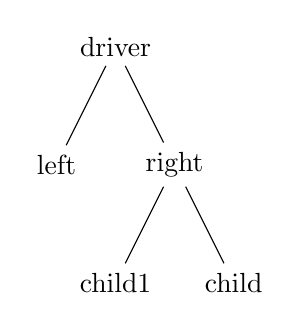
\begin{tikzpicture}
    \node {driver}
    child {node {left}}
    child {node {right}
    child {node {child1}}
    child {node {child}}
    };
\end{tikzpicture}

\begin{tikzpicture}
    %\fill [black!20] (0,0) rectangle (4,4);
    %\path [pattern=checkerboard,pattern color=black!30] (0,0) rectangle (4,4);

    \shade [ball color=blue,path fading=south] (2,3) circle (1.8);
\end{tikzpicture}

\includegraphics[width=4in]{vfs.ps}

\vskip .5cm
1}}}
\end{comment}

%%%%%%%%%%%%%%%%%%%%%%%%%%%%%%%%%%%%%%%%%%%%%%%%%%%%%%%%%%%%%%%%%%%%%%%%%%%%%
%%%%%%%%%%%%%%%%%%%%%%%%%%%%%%%%%%%%%%%%%%%%%%%%%%%%%%%%%%%%%%%%%%%%%%%%%%%%%
\begin{comment}
E/dumpsys (  514):  service: SurfaceFlinger
E/BpBinder(  514): do transact
D/IPCThreadState ipc(  514): >>>> SEND from pid 514 uid 0 READ REPLY
W/IPCThreadState (  514): in waitForResponse before talkWithDriver
W/IPCThreadState (  514): before ioctl(xxx, BINDER_WRITE_READ
W/IPCThreadState (  514): after ioctl(xxx, BINDER_WRITE_READ
W/IPCThreadState (  514): Processing waitForResponse Command: unknown
W/IPCThreadState (  514): in waitForResponse before talkWithDriver
W/IPCThreadState (  514): Processing waitForResponse Command: unknown
W/IPCThreadState (  514): in waitForResponse before talkWithDriver
W/IPCThreadState (  514): Processing waitForResponse Command: unknown
I/IPCThreadState (  514): >>>>>> return transact from waitForResponse 
V/BpBinder(  514): Creating BpBinder 0xbd58 handle 1
D/IPCThreadState remoterefs(  514): IPCThreadState::incWeakHandle(1)
V/BpBinder(  514): onFirstRef BpBinder 0xbd58 handle 1
D/IPCThreadState remoterefs(  514): IPCThreadState::incStrongHandle(1)
E/dumpsys (  514): do pingBinder()
E/BpBinder(  514): do pingBinder
E/BpBinder(  514): do transact
D/IPCThreadState ipc(  514): >>>> SEND from pid 514 uid 0 READ REPLY
W/IPCThreadState (  514): in waitForResponse before talkWithDriver
W/IPCThreadState (  514): before ioctl(xxx, BINDER_WRITE_READ
W/IPCThreadState (   95): after ioctl(xxx, BINDER_WRITE_READ
W/Binder  (   95): reached BBinder::transact (this=0x969fc), code=1599098439
W/Binder  (   95): reached BBinder::pingBinder (this=0x969fc)
D/IPCThreadState ipc(   95): Sending reply to 514!
I/IPCThreadState (   95): >>>>>> call waitForResponse in sendReply 
W/IPCThreadState (   95): in waitForResponse before talkWithDriver
W/IPCThreadState (   95): before ioctl(xxx, BINDER_WRITE_READ
W/IPCThreadState (   95): after ioctl(xxx, BINDER_WRITE_READ
W/IPCThreadState (   95): Processing waitForResponse Command: unknown
W/IPCThreadState (   95): in waitForResponse before talkWithDriver
W/IPCThreadState (   95): Processing waitForResponse Command: unknown
W/IPCThreadState (   95): before ioctl(xxx, BINDER_WRITE_READ
W/IPCThreadState (  514): after ioctl(xxx, BINDER_WRITE_READ
W/IPCThreadState (  514): Processing waitForResponse Command: unknown
W/IPCThreadState (  514): in waitForResponse before talkWithDriver
W/IPCThreadState (  514): Processing waitForResponse Command: unknown
W/IPCThreadState (  514): in waitForResponse before talkWithDriver
W/IPCThreadState (  514): Processing waitForResponse Command: unknown
I/IPCThreadState (  514): >>>>>> return transact from waitForResponse 
V/BpBinder(  514): onLastStrongRef BpBinder 0xbd58 handle 1
D/IPCThreadState remoterefs(  514): IPCThreadState::decStrongHandle(1)
V/BpBinder(  514): Destroying BpBinder 0xbd58 handle 1
D/IPCThreadState remoterefs(  514): IPCThreadState::decWeakHandle(1)
V/BpBinder(  514): Killing 0 objects in manager 0xbd70
V/BpBinder(  514): onLastStrongRef BpBinder 0xb370 handle 0
D/IPCThreadState remoterefs(  514): IPCThreadState::decStrongHandle(0)
V/BpBinder(  514): Destroying BpBinder 0xb370 handle 0
D/IPCThreadState remoterefs(  514): IPCThreadState::decWeakHandle(0)
# V/BpBinder(  514): Killing 0 objects in manager 0xb388

 kpsewhich mpost.mem

/usr/share/texmf-texlive/metafont/base/
Sorry, I can't find the 'mpost' mem file; will try 'plain'.
mpost -ini '\input plain dump'


>> extra_beginfig
>> "boxjoin();save pic_,sproc_,pproc_;def clearboxes=enddef;"
! Not implemented: (unknown numeric)&(string).

xu@xu-laptop:~/work$  mpost -ini '\input mpost dump'
This is MetaPost, version 1.208 (kpathsea version 5.0.0) (INIMP)
! I can't find file `mpost'.
<*> \input mpost
                 dump
Please type another input file name: plain
... ...
and a few last-minute items.)
Beginning to dump on file mpost.mem
 (mem=mpost 2012.05.09)
at most 828 strings of total length 4732
4600 memory locations dumped; current usage is 1226&3259
570 symbolic tokens
Transcript written on mpost.log.

plain -> mpost.mem, 这个mpost.mem是有问题的, 而mpost.mem 又是先搜索的。
删除之即可。


xu@xu-laptop:~/work$  mpost -ini '\input mpost dump'
This is MetaPost, version 1.208 (kpathsea version 5.0.0) (INIMP)
(/usr/share/texmf-texlive/metapost/base/mpost.mp
(/usr/share/texmf-texlive/metapost/base/plain.mp
安装feynmf, texlive-metapost之后,才有mpost.mp,才可以生成mpost.mem.
metauml 也是在这个包里的。


latexmk, 把 /usr/bin/latexmk $latex  = 'xelatex';
latexmk foo.mp

\end{comment}
%%%%%%%%%%%%%%%%%%%%%%%%%%%%%%%%%%%%%%%%%%%%%%%%%%%%%%%%%%%%%%%%%%%%%%%%%%%%%
%%%%%%%%%%%%%%%%%%%%%%%%%%%%%%%%%%%%%%%%%%%%%%%%%%%%%%%%%%%%%%%%%%%%%%%%%%%%%
\end{document}
